%% -----------------------------------------------------------------
%% This file uses UTF-8 encoding
%%
%% For compilation use following command:
%% latexmk -pdf -pvc -bibtex thesis
%%
%% -----------------------------------------------------------------
%%                                     _     _
%%      _ __  _ __ ___  __ _ _ __ ___ | |__ | | ___
%%     | '_ \| '__/ _ \/ _` | '_ ` _ \| '_ \| |/ _ \
%%     | |_) | | |  __/ (_| | | | | | | |_) | |  __/
%%     | .__/|_|  \___|\__,_|_| |_| |_|_.__/|_|\___|
%%     |_|
%%
%% -----------------------------------------------------------------

\documentclass{kithesis}
% Please add the following required packages to your document preamble:
% Additional packages
\usepackage[main=slovak,english]{babel}
% For thesis written in English just change the order of languages:
% \usepackage[main=english,slovak]{babel}

\usepackage{listings}  % for source code
% Listings settings
% See for details: https://en.wikibooks.org/wiki/LaTeX/Source_Code_Listings
\lstset{
    basicstyle=\small\ttfamily,  % smaller typewriter font
    showstringspaces=false       % don't show spaces in string
}

% Location of file with bibliography resources
\addbibresource{chapters/bibliography.bib}

% Variables
%\thesisspec{figures/thesisspec.png}
\title{My thesis \br (the skeleton)}{Riešenie úloh strojového učenia \br využitím Kubernetes}

%\author{Janko Hraško}
\author{Štefan}{Hadbavný}
\supervisor{Marek Ružička} %veduci prace
\consultant{Marcel Vološin} %konzultant
%\college{University of Žilina}{Žilinská univerzita} %univerzita
%\faculty{Faculty of Electrical Engineering and informatics}{Fakulta elektrotechniky a informatiky} %fakulta
%\department{Department of Computers and Informatics}{Katedra počítačov a informatiky} %katedra
%\departmentacr{DCI}{KPI} % skratka katedry
%\thesis{Master thesis}{Diplomová práca} %typ prace
\submissiondate{13}{5}{2022}
%\fieldofstudy{9.2.1 Informatika}
%\studyprogramme{Informatika}
%\city{Košice} %mesto
\keywords{Kubernetes, Kubeflow, Machine learning, Containerization}{Kubernetes, Kubeflow, Strojové učenie, Kontajnerizácia}
%\declaration{som nepodvadzal}

\abstract{%
    % english
	The main goal of this work is to create a Kubernetes test environment with the possibility running machine learning tasks. The first part is devoted to terminology and architecture of Kubernetes platform and containerization. The analysis is followed by a structure of the main components of the Kubeflow platform and the definition of scenarios for creation test environments composed of Kubernetes and Kubeflow platforms. Last but not least is made a comparison of scenario deployments, their advantages and disadvantages. A table has been prepared for a clear summary of implementations requirements. Attached is a manual for creating a test center using Kubernetes and a user guide for implementing Python tasks.

}{%
    % slovak
	Hlavným cieľom práce je vytvoriť testovacie prostredie Kubernetes s možnosťou spúšťania úloh strojového učenia. Prvá časť je venovaná terminológii, architektúre platformy Kubernetes a kontajnerizácii. Po analýze nasleduje rozbor hlavných komponentov platformy Kubeflow a definovanie scenárov pre vytvorenie testovacích prostredí zložených z Kubernetes a Kubeflow platforiem. V poslednom rade je zhotovené porovnanie nasadení scenárov, ich výhody a nevýhody.  Vypracovaná bola tabuľka pre prehľadný súhrn požiadaviek, výhod a nevýhod implementácií. V prílohe je priložený manuál na vytvorenie testovacieho prostredia využitím Kubernetes a používateľská príručka na implementáciu Python úloh.
}
\thesisspec{figures/zadavaci-list.png}

\acknowledgment{Vyhlasujem úprimné poďakovanie môjmu vedúcemu práce Ing. Marekovi Ružičkovi a konzultantovi Ing. Marcelovi Vološinovi PhD. za odbornú pomoc, cenné rady a čas, ktorý mi venovali pri písaní tejto bakalárskej práce.

Rovnako by som sa rád poďakoval portálu CLOUD TUKE za poskytnutie virtuálnych strojov a pomoci pri konfigurácii.}

% if you want to work only on selected chapters
%\includeonly{chapters/analyza} %,chapters/synteza}

% Load acronyms
% Acronyms
% ========
%
% An acronym is a word formed from the initial letters in a phrase.
%
% Acronym Definition Exapmle:
% ---------------------------
% \newacronym{gcd}{GCD}{Greatest Common Divisor}
% \newacronym{dry}{DRY}{Don't Repeat Yourself}
%
% Usage:
% ------
% You can use these three options:
%
% \acrlong{}
%   Displays the phrase which the acronyms stands for. Put the label of the acronym inside the braces. In the example, \acrlong{gcd} prints Greatest Common Divisor.
%
% \acrshort{}
%   Prints the acronym whose label is passed as parameter. For instance, \acrshort{gcd} renders as GCD.
%
% \acrfull{ }
%   Prints both, the acronym and its definition. In the example the output of \acrfull{dry} is Don't Repeat Yourself (DRY).
%
% For more information see:
% -------------------------
% * https://www.sharelatex.com/learn/Glossaries
% * https://en.wikibooks.org/wiki/LaTeX/Glossary
%


\newacronym{rest}{REST}{Representational State Transfer}
\newacronym{api}{API}{Application Programming Interface}
\newacronym{it}{IT}{Information Technology}
\newacronym{udp}{UDP}{User Datagram Protocol}
\newacronym{tcp}{TCP}{Transmission Control Protocol}
\newacronym{sctp}{SCTP}{Stream Control Transmission Protocol}
\newacronym{http}{HTTP}{Hypertext Transfer Protocol}
\newacronym{ui}{UI}{User Interface}
\newacronym{json}{JSON}{JavaScript Object Notation}
\newacronym{yaml}{YAML}{Ain't Markup Language}
\newacronym{iot}{IOT}{Internet of things}
\newacronym{dns}{DNS}{Domain Name System}
\newacronym{wsl}{WSL}{Windows Subsystem for Linux}
\newacronym{unix}{UNIX}{Uniplexed Information and Computing Service}
\newacronym{sdk}{SDK}{Software Development Kit}
\newacronym{ip}{IP}{Internet Protocol}
\newacronym{url}{URL}{Uniform Resource Locator}
\newacronym{ssh}{SSH}{Secure Shell Protocol}
\newacronym{socks}{SOCKS}{Windows Sockets}
\newacronym{mac}{MAC}{Media Access Control Address}
\newacronym{cni}{CNI}{Common Network Interface}
\newacronym{apt}{APT}{Advanced Packaging Tool}
\newacronym{k8s}{K8S}{Kubernetes}



%% -----------------------------------------------------------------
%%          _                                       _
%%       __| | ___   ___ _   _ _ __ ___   ___ _ __ | |_
%%      / _` |/ _ \ / __| | | | '_ ` _ \ / _ \ '_ \| __|
%%     | (_| | (_) | (__| |_| | | | | | |  __/ | | | |_
%%      \__,_|\___/ \___|\__,_|_| |_| |_|\___|_| |_|\__|
%%
%% -----------------------------------------------------------------
\usepackage{multirow}
\begin{document}
%% Title page, abstract, declaration etc.:
\frontmatter{}

%% List of code listings, if you are using package minted
%\listoflistings

%\pagenumbering{arabic}

%% Chapters
% !TEX root = ../thesis.tex

\chaptermark{Úvod}
\phantomsection
\addcontentsline{toc}{chapter}{Úvod}

\chapter*{Úvod}

Strojové učenie v dnešnej dobe veľmi rýchlo napreduje. Je dôležitou súčasťou rastúcej oblasti vedy o údajoch. Pomocou štatistických metód sú algoritmy trénované na vytváranie klasifikácií alebo predpovedí, ktoré odhaľujú kľúčové poznatky v rámci rôznych projektov. Tieto poznatky následne riadia rozhodovanie, čo v ideálnom prípade ovplyvňuje kľúčové metriky. Vyžaduje sa od nich, aby pomáhali pri identifikácii najrelevantnejších otázok a následne údajov, ktoré by na nich odpovedali. Pri experimentoch strojového učenia je niekedy vyžadovaný vyšší výkon. Ak sú prístupné viaceré stroje, ktoré sú rozdelené medzi viacerými používateľmi a na danom počítači je žiadaný vyšší výkon, migrovanie údajov manuálne medzi strojmi by bolo zdĺhavé. Ideálnym riešením je, aby Kubernetes bežal na strojoch a nasadzovali by sa naň úlohy bez toho, aby sa muselo riešiť na ktorom stroji sa spustia.

Riešenie úloh strojové učenia sa stáva bežne implementovaným nástrojom na uľahčenie pracovnej záťaže zamestnancov a vedcom v rôznych oblastiach, od kybernetickej bezpečnosti až po služby zákazníkom. Možným riešením, ktoré môže priniesť výhody, je open-source technológia kontajnerizácie Kubernetes. Umožňuje rýchlu, jednoduchú správu a prehľadnú organizáciu kontajnerových služieb a aplikácií. Táto technológia tiež umožňuje automatizáciu prevádzkových úloh, ako je správa dostupnosti aplikácií a škálovanie. Podporuje GPU, čo urýchľuje pracovný tok a automatizuje správu kontajnerov aplikácií akcelerovaných GPU. Tieto nástroje umožňujú využiť rýchlosť GPU v rámci kontajnerového pracovného postupu.

Niekedy sú bežiace postupy na Kubernetes komplikované. Tento problém je možne vyriešiť nadstavbou Kubeflow. Pomáha efektívne spúšťať, organizovať a škálovať modely nezávisle od ich závislostí, ako často musia byť aktívne a koľko údajov potrebujú spracovať. Cieľom Kubeflow je uľahčiť inžinierom strojového učenia a vedcom využívať cloudové prostriedky pre pracovné zaťaženie strojového učenia. Dokáže efektívne vytvorenie modelu pripraveného na produčné použitie za veľmi krátky čas.

Existuje veľa distribútorov, firiem, ktoré vyvíjajú tieto platformy a sú rôzne prispôsobované, preto je cieľom tejto práce otestovať jednotlivé spôsoby a možnosti týchto nasadení. Je potrebné zohľadňovať viaceré faktory. Faktory ako sú podpora grafickej karty, možnosť prepojenia viacerých strojov, systémové požiadavky alebo softverové rámce.

Vyber správnej implementácie je dôležitý. Mala by mať čo najmenej problémov s ktorými sa autor tejto práce stretne a poskytovala čo najlepšie hardvérové využitie.

\section*{Formulácia úlohy}

Hlavnou úlohou tejto práce je vytvoriť testovacie prostredie Kubernetes s možnosťou spúšťania úloh strojového učenia naprogramovaných v jazyku Python. Najprv je vhodné venovať pozornosť analýze tejto platformy. Platforma Kubernetes je na prvý pohlaď náročná, taktiež vďaka rôznym výrazom, ktoré s ňou súvisia. Na mieste je opis týchto komponentov, architektúry a kontajnerizaciu, pre lepšie pochopenie tejto platformy pre používateľa. Otestovanie nasadení využitím rôznych nástrojov, ktoré je možné otestovať a vyhodnotiť. Uskutočniť prepojenie viacerých počítačov v klastri a odskúšať funkčnosť podpory grafickej karty. Po testovaní je na rade porovnanie a vyhodnotenie jednotlivých scenárov a výber najlepšieho nasadenia vhodného na vyriešenie danej problematiky. V poslednom rade je vyhotovenie manuálu na vytvorenie a pripojenie viacerých počítačov do platformy Kubernetes a manuál (sériu pokynov s príkladmi) na implementáciu a nasadenie Python zdrojových kódov spustiteľných na platforme Kubernetes.
% !TEX root = ../thesis.tex

\chapter{Analytická časť}
Pri strojovom učení a experimentoch je niekedy potreba na krátku dobu vyšší výkon. Pravidelné migrovanie medzi strojmi by bolo veľmi zdĺhavé. S tým nám pomôže platforma kubernetes.

Kubernetes je platforma, ktorá je veľmi robustná v nasadení, správe a orchestrácií kontajnerov. Dokáže rozdeliť súčasne záťaž medzi jednotlivými strojmi. Tato platforma v súčasnosti vytlačila predošle platformy a stala sa už štandardom. Nasadenie Kubernetes je najefektívnejšie, aj keď existuje dnes veľa podobných technológii a mnoho významných poskytovateľov ponúka klastre Kubernetes.

Podľa mojich uvážení je na našu problematiku vhodný Kubeflow.

\section{Kubernetes}
Spôsob, akým je Kubernetes navrhnutý, je to, čo ho robí výnimočným. Kubernetes má základnú architektúru klienta a servera. Kubernetes má schopnosť vykonávať priebežné aktualizácie, prispôsobuje sa aj ďalším pracovným zaťaženiam automatickým škálovaním uzlov, ak je to potrebné, a môže sa tiež opraviť v prípade rozpadu podu. Poskytujú obrovskú výhodu v tom, že aplikácie nebudú mať žiadne výpadky.

Ako orchestrátor sa stará o prácu s plánovaním kontajnerov v klastri a tiež spravuje pracovné zaťaženia. Takmer všetko v Kubernetes používa deklaratívne konštrukty, ktoré popisujú, ako sa aplikácie skladajú, ako interagujú a ako sú spravované.

Táto platforma je vhodná na riešenie úloh strojového učenia, aj keď priamo na to je vyvinutý kubeflow, Je najrýchlejšie rastúcim projektom z Open Source softvéru. Kubernetes je vhodný na riešenie hlavne kvôli týmto výhodám:

\subsection*{Prenosnosť}
Ponúka prenosnosť, rýchlejšie a jednoduchšie nasadenie. To znamená, že v prípade potreby využívať výhody viacerých cloudov alebo serverov a môžu sa rýchlo rozvíjať bez toho aby sa musela meniť infraštruktúru.

\subsection*{Škálovateľnosť}
Ma schopnosť spúšťať kontajnery na jednom alebo viacerých verejných cloudových prostrediach, vo virtuálnych strojoch, čiže je ho možné nasadiť takmer kdekoľvek. A keďže Kubernetes zásadne zmenil spôsob vývoja a nasadzovania, je možné škálovať oveľa rýchlejšie, než v minulosti.

\subsection*{Dostupnosť}
Rieši vysokú dostupnosť na úrovni aplikácie aj infraštruktúry. Pridanie spoľahlivej úložnej vrstvy do Kubernetes zaisťuje vysokú dostupnosť stavových úloh. Okrem toho môžu byť hlavné komponenty klastra nakonfigurované na multi-node replikáciu (multi-master), čo tiež zabezpečuje vyššiu dostupnosť.

\subsection{Architektúra}
Pracovné uzly (worker), hlavný uzol (master) a spolu s API, tvoria architektúru Kubernetes. V tejto časti je opísaná architektúra ako tieto uzly fungujú a načo slúži API.

Je zložený z niekoľkých častí, ktoré sú potrebné pre jeho správne fungovanie a efektivitu. Pre správne pochopenie ako Kubernetes funguje je treba sa zoznámiť najmä s niektorými termínmi.

V hlavnom uzle nájdeme komponenty, ktoré riadia klaster spolu s údajmi o stave a konfigurácii klastra. Tieto základne komponenty pracujú tak aby dokázali zabezpečiť prácu tak aby kontajnery fungovali v dostatočnom počte a spotrebnými zdrojmi.
Hlavný uzol je neustále v kontakte s jednotlivými strojmi, ktoré vykonávajú prácu. Hlavný uzol sa postará o klaster, tak ako sme ho nakonfigurovali.



\subsection*{Mikroslužby}
Pre mikroslužby neexistuje presná definícia. Často sa používajú pri cloudových službách a aplikácii, ktoré sa nasadzujú pomocou kontajnerov.  

\subsection*{Uzol}
Uzol môže byt virtuálny stroj alebo fyzicky počítač, kde sú nasadené kontajnery. Za prijímanie a spúšťanie pracovných zaťažení a externých zdrojov sú zodpovedne uzly. Kubernetes spúšťa aplikácie a služby v kontajneroch na pomoc s izoláciou, správou a flexibilitou. Každý uzol musí mat modul tzv. runtime kontajnera. Uzol prijíma pracovne pokyny od hlavného uzla a podlá toho vytvára alebo ruší kontajnery a zároveň prispôsobuje pravidla sieťovej prevádzky.

\subsection*{Pod}
Pod je skupina jedného alebo viacerých kontajnerov so zdieľaným úložiskom, sieťou a špecifikáciou ako majú kontajnery fungovať. Pri necloudových sú spúšťane na rovnakom fyzickom alebo virtuálnom stroji a pri cloudových na rovnakom logickom hostiteľovi. Všetky kontajnery v pode môžu medzi sebou komunikovať aj sú na samostatných uzloch. Sú vytvorené na základe pracovného zaťaženia nazývanými ovládače, ktoré riadia vytváranie, kopírovanie a stav podov v klastri. Ak napríklad zlyhá uzol v klastri, ovládač zisti, že moduly v tomto uzle nereagujú a vytvorí náhradne moduly na iných uzloch.

\subsection*{Klaster}
V klastroch sa spúšťajú kontajnerové aplikácie, ktoré spravuje Kubernetes. Klaster je v podstate séria uzlov spojených dohromady. Spojením uzlov zhromažďujú svoje zdroje(CPU, RAM, atď.). Klaster je v tom prípade oveľa výkonnejší ako jednotlivé stroje. Kubernetes presúva pody po klastri, pri pridávaní alebo odstraňovaní uzlov.\cite{kubernetes2} Sú to navzájom prepojene počítače, ktoré vykonávajú určitú činnosť.

\subsection*{Kontajner}
Kontajner je podobný virtuálnemu stroju ale kontajner je viac efektívnejší, podobne ako virtuálny stroj ma vlastný súborový systém, zdieľaný procesor, operačnú pamäť a ďalšie. Sú funkčne na rôznych operačných systémoch, pretože sa oddeľujú od základnej infraštruktúry.\cite{kubernetes}
Výrazne zvyšujú efektivitu, vyžadujú menej systémových prostriedkov, pretože neobsahujú obraz operačného systému. Zabezpečujú lepší vývoj aplikácii a lepšiu prenosnosť.

\subsection*{Kube-apiserver}
Tento komponent odhaľuje API hlavnému uzlu. V podstate funguje ako frontend k informáciám o stave klastra a premosťuje API s inými objektmi Kubernetes, napríklad modulmi, radičmi a službami. Server API určuje, ci je požiadavka platná, a ak áno, spracuje ju. K API sa pristupuje prostredníctvom Rest, cez rozhranie príkazového riadka kubectl alebo prostredníctvom iných nástrojov napríklad kubeadm. Zabezpečuje všetku interakciu medzi komponentmi.\cite{kubeapiserver}

\subsection*{Kube-controller-manager}
Na hlavnom uzle riadi všetky ovládače. Každý ovládač je vlastne samostatný individuálny proces. Pre zjednodušenie správy klastrov sú však všetky skompilovane do jedného procesu, Za tuto kompiláciu je zodpovedný kube-controller-manager. Jeden ovládač konzultuje plánovač a uisťuje sa, že beží správny počet podov. Ak pod spadne, iný ovládač si to všimne a zareaguje. Ovládač pripája služby k podom, takže požiadavky smerujú do správneho koncového bodu. Existujú aj ovládače na vytváranie účtov a prístupových tokenov API.\cite{kubecontroler}

\subsection*{Etcd}
Ukladá informácie o konfigurácii pre veľké distribuovane systémy  Kubernetes teda používa etcd ako úložisko hodnôt jednotlivých kľúčov. Etcd modul musí byt stále dostupný, aby sa zabezpečilo správne fungovanie služieb. Údaje Etcd sú veľmi doležíte a odporúča sa vytvoriť si zálohu. 

\subsection*{Plánovač}
Z názvu môžeme posúdiť, že slúži na plánovanie rozhodnutí pre novovytvorené pody. Keď je pod vytvorený, musí mu byť priradený uzol, na ktorom sa má spustiť. Plánovač prijíma informácie z API o požiadavkách a špecifikáciách podov a IT zdrojoch na dostupných uzloch. Potom priradí každý pod k príslušnému uzlu. Ak plánovač nemôže nájsť vhodný uzol, pod zostane nenaplánovaný a plánovač zopakuje proces, kým nebude dostupný uzol.

\subsection*{}
Komponent, ktorý sa nasadzuje ako prvý je takzvaný runtime kontajnera. Zvyčajne sa inštaluje spustením Dockera, ale dostupné sú aj alternatívy ako rkt a runc.
Runtime kontajnera je zodpovedný za spustenie a správu kontajnerov, aplikácií zapuzdrených v relatívne izolovanom, ale ľahkom ako keby operačnom prostredí. 

Každá jednotka práce v klastri je na svojej základnej úrovni implementovaná ako jeden alebo viac kontajnerov, ktoré je potrebné nasadiť. 

\subsection*{Kubelet}
Kubelet je agent, ktorý je spustený na každom pracovnom uzle v klastri. Je to dôležitý komponent, pretože prijíma inštrukcie z hlavného uzla. Kubelet v podstate riadi pody. Zabezpečuje, že všetky kontajnery bežia v pode a že tieto pody sú v poriadku a bežia v správnych časových intervaloch. Číže vytvára a odstraňuje moduly, na základe pokynov od hlavného uzla, ktoré moduly je potrebné pridať alebo odstrániť. Keď riadiaci uzol potrebuje, aby sa niečo vykonalo v uzle, kubelet vykoná tuto akciu.

\subsection*{Kube-proxy}
Na správu jednotlivých hostiteľských podsietí a sprístupnenie služieb iným komponentom je na každom uzlovom serveri spustená malá proxy služba s názvom kube-proxy . Tento proces preposiela požiadavky správnym kontajnerom, môže vykonávať primitívne vyvažovanie záťaže a je vo všeobecnosti zodpovedný za zabezpečenie toho, aby bolo sieťové prostredie predvídateľné a dostupné, ale v prípade potreby izolované. Používa proxy UDP, TCP a SCTP, ale nerozumie HTTP.

\subsection*{}
Na obrázku môžeme vidieť jednotlivé komponenty:
\begin{figure}[!ht]
    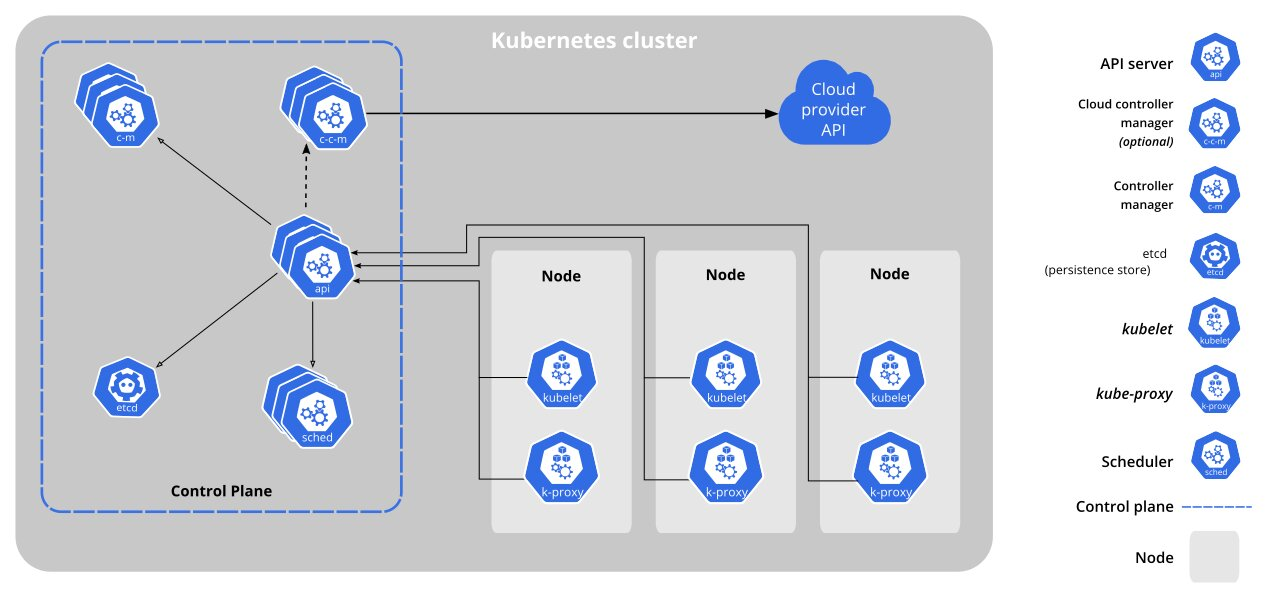
\includegraphics[width=.9\textwidth]{figures/kubernetesarchi}
    \caption{\ Architektúra kubernetes \cite{archkuber} \label{o:latex_friendly_zone}}
\end{figure}

\subsection{Nástroje}

Nástroje slúžia na vytváranie lokálneho klastra a následne pracovanie s týmto klastrom. V tejto časti si porovnane nástroje aké majú odlišnosti a čo ponúkajú.
\subsection*{minikube}

Ide o spôsob vytvárania virtuálneho počítača, ktorý je v podstate klastrom Kubernetes s jedným uzlom. Vďaka podpore množstva hypervízorov ho možno použiť na všetkých hlavných operačných systémoch. To tiež umožňuje vytvárať viacero inštancií paralelne.

Z užívateľského hľadiska je minikube veľmi priateľský nástroj pre začiatočníkov. Klaster sa spúšťa pomocou minikube start, následne kubectl je pripravený na použitie. Na určenie verzie Kubernetes sa používa príkaz --kubernetes-version.

Pre nových používateľov Kubernetes, môže výrazne pomôcť dashboard, ktorý minikube ponúka. Dashboard sa jednoducho otvorí a poskytuje pekný prehľad o všetkom, čo sa deje v klastri. Minikube taktiež umožňuje pridávať rôzne rozšírenia, ktoré pomáhajú integrovať napríklad dashboard, grafické karty od Nvidie a oveľa viac. Pomocou minikube sa vykonávajú príkazy ako vytvoriť, aktualizovať, odstrániť klaster lokálne na počítači. Je užitočný, pre rýchle vytvorenie malého testovacieho klastera. Používa celkom jednoduché príkazy na vytvorenie a odstránenie klastra.

\subsection*{kind}

Ako už názov napovedá, presúva klaster do kontajnerov Docker. To vedie k výrazne vyššej rýchlosti spustenia v porovnaní s vytváraním virtualizácie.

Vytvorenie klastra je veľmi podobné ako pri minikube. Použitím príkazu kind create cluster, vytvárame klaster. Použitím rôznych názvov  --name, kind umožňuje vytvárať viaceré inštancie paralelne.

Jedna funkcia, ktorá sa mi osobne páči, je možnosť načítať obrazy kontajnerov priamo do klastra. To ušetrí niekoľko ďalších krokov pri nastavovaní registra a načítavaní môjho obrazu, keď chcem vyskúšať nejaké zmeny. S jednoduchým kind load docker-image my-app:latest je kontajnerový obraz k dispozícii na použitie v mojom klastri.

\subsection*{k3s}

K3s je verzia Kubernetes vyvinutá spoločnosťou Rancher Labs. Odstránením postradateľných funkcií (legacy, in-tree pluginy) a použitím ľahkých komponentov (napr. sqlite3 namiesto etcd3) dosiahli výrazné zmenšenie. Výsledkom je jeden binárny súbor s veľkosťou približne 60 MB.

Aplikácia je rozdelená na server K3s a agenta. Prvý pôsobí ako manažér, zatiaľ čo druhý zodpovedá za zvládnutie skutočného pracovného zaťaženia. Upozorňujem, že pri spúšťaní na počítací môže dôjsť k výraznému neporiadku v lokálnom súborovom systéme. Namiesto toho sa vkladá k3s do kontajnera (napr. pomocou rancher/k3s), ktorý tiež umožňuje ľahko spustiť niekoľko nezávislých inštancií.

Jedna funkcia, ktorá vyniká, sa nazýva automatické nasadenie. Umožňuje nasadiť manifesty Kubernetes a grafy Helm ich umiestnením do konkrétneho adresára. K3s sleduje zmeny a stará sa o ich aplikáciu bez akejkoľvek ďalšej interakcie. Je to užitočné najmä pre CI pipelines a zariadenia lot. Stačí vytvoriť/aktualizovať konfiguráciu a K3s sa postará o to, aby boli nasadenia (deployments) aktuálne.

\subsection*{MicroK8s}
Sťahuje sa ako inštalačný balík, ktorý nainštaluje jednouzlový (samostatný) klaster K8s za menej ako 60 sekúnd. Da sa použiť aj na vytvorenie klastra s viacerými uzlami pomocou niekoľkých príkazov. MicroK8s má všetky základné komponenty Kubernetes, ako napríklad DNS a Dashboard, sú dostupné použitím jediného príkazu.

MicroK8s je k dispozícii pre väčšinu populárnych distribúcií Linuxu a tiež pre pracovné stanice Windows a Mac prostredníctvom natívneho inštalátora pre oba operačné systémy. V systéme Windows je tiež možnosť získať MicroK8s na WSL.

Používa snap packaging mechanizmus, čož je naozaj pohodlné, pretože prináša automatické aktualizácie. To znamená, že akonáhle bude k dispozícii nová stabilná verzia Kubernetes, váš klaster MicroK8s sa automaticky aktualizuje. Podobne sa získavajú všetky dostupné bezpečnostné záplaty pre Kubernetes.\cite{comparetool}

\subsection*{}

Každý z týchto nástrojov poskytuje ľahko použiteľné prostredie Kubernetes pre viacero platforiem, no odlišujú ich niekoľko faktorov.

K3s napríklad ponúka prostredie Kubernetes založené na virtualizácii. Pre nastavenie viacero serverov Kubernetes, je potreba manuálne nakonfigurovať ďalšie virtuálne stroje alebo uzly, čo môže byť dosť náročné. Je však navrhnutý na použitie pri nasadzovaní, čo z neho robí jednu z najlepších možností na lokálne simulovanie skutočného nasadzovacieho prostredia.

Aj keď je minikube vo všeobecnosti skvelou voľbou pre lokálne spúšťanie Kubernetes, jednou z hlavných nevýhod je, že môže spustiť iba jeden uzol v miestnom klastri, čo zas vyúsťuje k tomu, zem je o niečo ďalej k produkčnému multiuzlovému prostrediu.

Na rozdiel od miniKube môže microK8S prevádzkovať viacero uzlov v lokálnom klastri.

Inštalácia microK8S na počítače so systémom Linux, ktoré nepodporujú balík snap, je náročná v porovnaní s inými nástrojmi v tomto zozname. microK8S používa balík snap vytvorený spoločnosťou canonical na inštaláciu strojového nástroja Linux, čo sťažuje spustenie na distribúciách Linuxu, ktoré ho nepodporujú. miniKube sa tiež inštaluje na viacero platforiem pomocou virtualizácie.


\section{Kubeflow}
Kubeflow ako platforma, je vhodná na nasadenie a vývoj strojového učenia. Primárne slúži pre inžinierov a vedcov, ktorý pracujú s dátami. Obsahuje viaceré komponenty, z ktorých si vývojári môžu vybrať, čo je pre ich používateľov najlepšie, čo znamená, že na nasadzovanie nie je potrebný každý jeden komponent.\cite{web}
\subsection{Architektúra}

Stavia na platforme Kubernetes ako systéme na nasadenie, škálovanie a správu zložitých systémov. Pomocou konfiguračných rozhraní Kubeflow, môžeme špecifikovať nástroje strojového učenia, potrebné pre náš pracovný postup. Potom môžeme nasadiť pracovný postup do rôznych cloudov, miestnych platforiem na experimentovanie a na produkčné použitie.\cite{web}

Na nasledujúcom obrázku môžte vidieť architektúru Kubeflow.

\begin{figure}[!ht]
    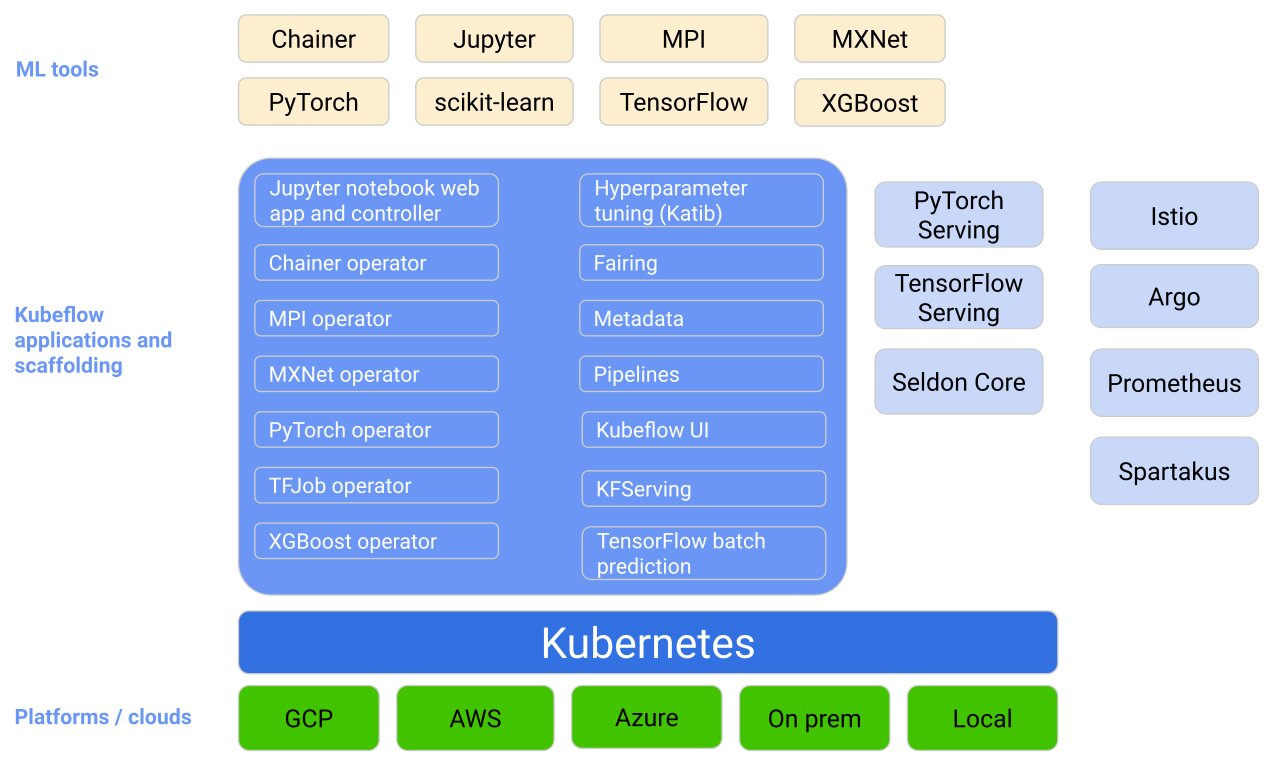
\includegraphics[width=.9\textwidth]{figures/kubeflowaarch}
    \caption{\ Architektúra kubeflow \cite{web} \label{o:latex_friendly_zone}}
\end{figure}

\subsection{Pracovný postup}
Postup pozostáva z viacerých krokov, taktiež z iterácie, ktorá je hlavným prvkom pri vyvíjaní sýtemu strojového učenia. Pri tomto postupe je potrebné vykonávať zmeny v parametroch aby sme dosiahli požadované výsledky.

Následne si povieme niečo viac o týchto postupoch.

Ako prvé by sme mali vyvíjať model na základe predpokladov a testov. Môžeme ho opísať v nasledujúcich bodoch:\cite{web}

\begin{itemize}
    \item Identifikovanie problému, ktorý ma systém vyriešiť.
    \item Zbieranie dát, ktoré potrebujeme na trénovanie modelu.
    \item Vyberanie algoritmu a nakódovanie modelu.
    \item Experiment s údajmi a trénovanie modelu.
	\item Vyladenie parametrov.
\end{itemize}

Ďalej môžeme nasadiť systém, ktorý bude vykonávať tieto procesy:

\begin{itemize}
    \item Transformáciu údajov, ktoré náš systém potrebuje.
	\item Trénovanie modelu.
	\item Podanie modelu na online prevádzku.
	\item Monitorovanie výsledkov na úpravu a zmenu modelu.
\end{itemize}
jkkjjkh
\begin{figure}[!ht]
    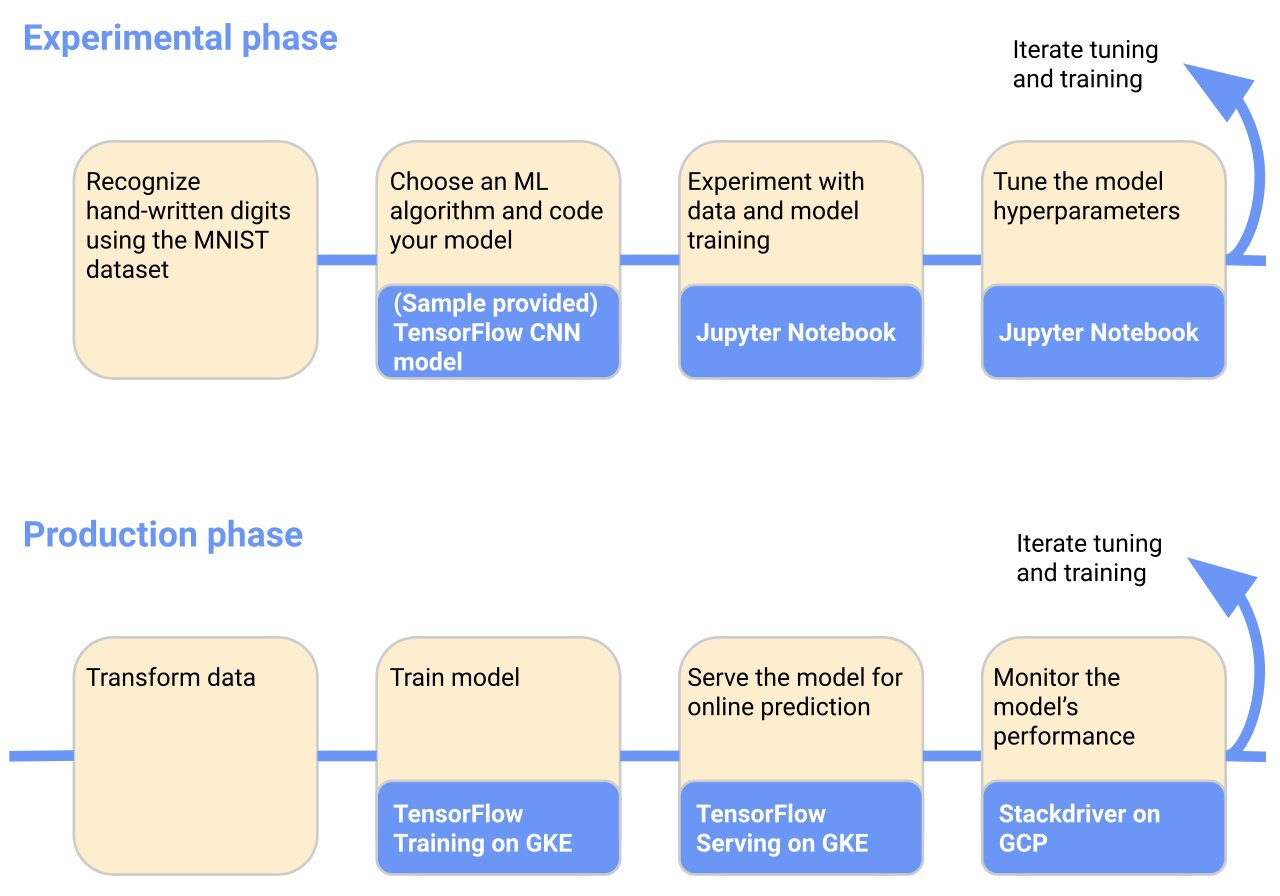
\includegraphics[width=.9\textwidth]{figures/kubeflowwork}
    \caption{\ Pracovné postupy \label{o:latex_friendly_zone}}
\end{figure}


\clearpage
\subsection{Rozhrania}

dopisaaat neskoor

\begin{figure}[!ht]
    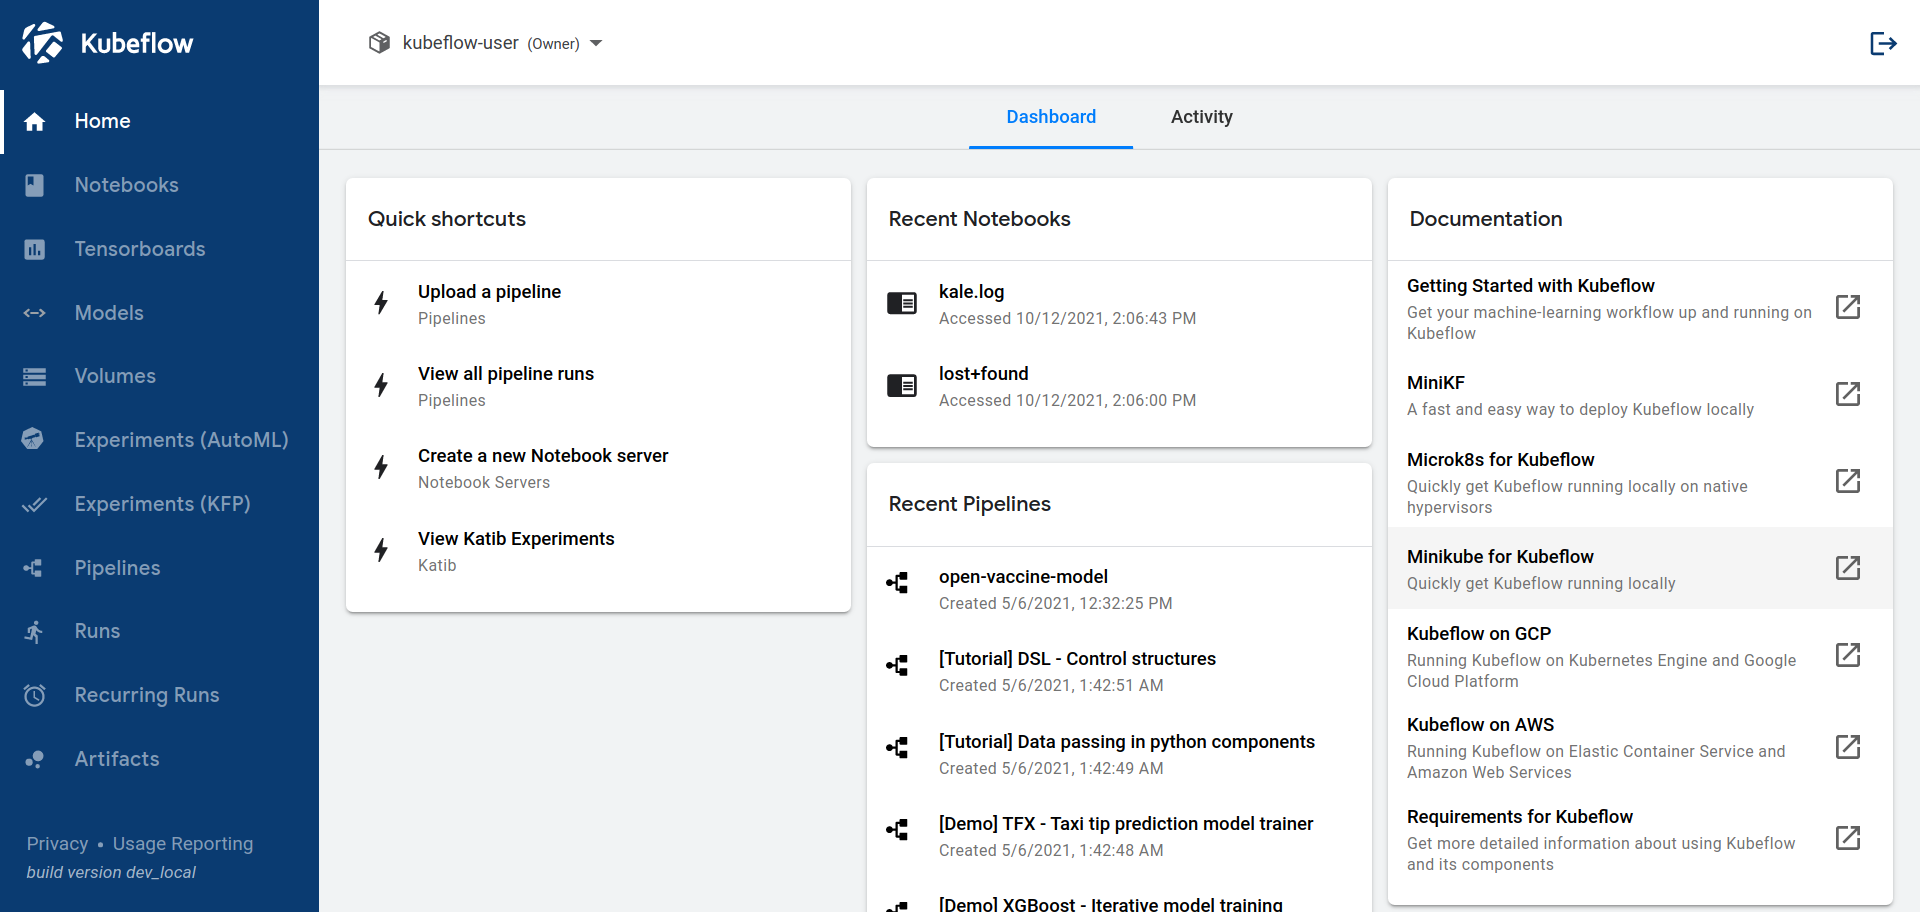
\includegraphics[width=.9\textwidth]{figures/Rozhranie}
    \caption{\ Rozhranie \label{o:latex_friendly_zone}}
\end{figure}

\clearpage
\section{Kontajnerizácia}

Kontajnery predstavujú metódu virtualizácie operačného systému, ktorá vám umožňuje spúšťať aplikáciu a jej závislosti v procesoch izolovaných na zdrojoch. Kontajnery nám umožňujú jednoducho zbaliť kód aplikácie, konfigurácie do ľahko použiteľných stavebných blokov, ktoré poskytujú environmentálnu konzistentnosť, prevádzkovú efektivitu, produktivitu vývojárov a kontrolu verzií. Kontajnery môžu pomôcť zabezpečiť rýchle, spoľahlivé a konzistentné nasadenie aplikácií bez ohľadu na prostredie nasadenia. Kontajnery tiež poskytujú podrobnejšiu kontrolu nad zdrojmi, čo zvyšuje efektivitu vašej infraštruktúry.

V minulosti sa aplikácie spúšťali na fyzických serveroch. Neexistovala možnosť ako nastaviť hranice pre aplikácie na serveroch a to spôsobovalo problémy. Napríklad, ak viaceré aplikácie bežali na jednom serveri, tak existovali tam inštancie, ktoré využívali väčšinu výkonu servera a ďalšie, ktoré nemali dostatočný výkon na vykonávanie akcii. To samozrejme sa už v dnešných časoch veľmi nevyužíva, tato metóda bola príliš nákladná na údržbu mnohých fyzických serverov.

Nasadzovanie aplikácie na virtualizovaných serveroch bolo predstavené ako riešenie. Umožňuje spustiť viacero virtuálnych strojov na jeden fyzicky server. Virtualizácia umožňuje izolovať aplikácie od seba a zabezpečiť tak, zem k informáciám jednej aplikácie sa nedostane druha aplikácia. Virtualizácia umožňuje lepšie využitie výkonu na serveri, aplikáciu umožňuje pridať, aktualizovať a taktiež znížene náklady na hardvér.

Kontajnery sú podobné virtuálnym počítačom, ale majú uvoľnené izolačné vlastnosti na zdieľanie operačného systému medzi aplikáciami. Preto sa kontajnery považujú za jednoduchšie. Podobne ako virtualizácia, kontajner má svoj vlastný súborový systém, zdieľané CPU, pamäte, procesného priestoru a ďalšie. Keďže sú oddelené od základnej infraštruktúry, sú prenosné cez cloudy a distribúcie operačných systémov.

Stali sa obľúbenými, pretože poskytujú veľa výhod:

\begin{itemize}
    \item Vyššia rýchlosť dodávania vylepšení. Kontajnerovanie monolitických aplikácií pomocou mikroslužieb pomáha vývojovým tímom vytvárať funkcie s vlastným životným cyklom a zásadami škálovania.
	\item Vylepšená bezpečnosť izoláciou aplikácií od hostiteľského systému a od seba navzájom.
	\item Nepretržitý vývoj, integrácia a nasadzovanie: poskytuje spoľahlivé a časté vytváranie a nasadzovanie obrazu kontajnera.
	\item Prenosnosť cloudu a distribúcie operačných systémov, na veľkých verejných cloudoch a kdekoľvek inde.
	\item Menšia záťaž. Kontajnery vyžadujú menej systémových prostriedkov ako tradičné alebo hardvérové prostredia virtuálnych strojov, pretože nezahŕňajú operačne systémy.
\end{itemize}

\subsection{Kontajnerový obraz, runtime a orchestrácia}

Súbory kontajnerového obrazu sú statické a spustiteľné verzie aplikácie alebo služby a líšia sa od jednej technológie k druhej. Obraz sa skladá z viacerých vrstiev, ktoré začínajú základným obrazom, ktorý obsahuje všetky závislosti potrebné na spustenie kódu v kontajneri. Každý obraz má na vrchu statických nemenných vrstiev čitateľnú a zapisovateľnú vrstvu. Pretože každý kontajner má svoju vlastnú špecifickú vrstvu kontajnera, ktorá prispôsobuje tento konkrétny kontajner, podkladové vrstvy obrazu možno uložiť a znova použiť vo viacerých kontajneroch. Pre otvorený kontajner sa obraz skladá z manifestu, vrstiev súborového systému a konfigurácií. Pre správne fungovanie kontajnera, musí mať runtime a špecifikáciu obrazu. Špecifikácie runtime predstavujú fungovanie súborového systému, čo sú súbory obsahujúce všetky potrebné údaje pre chod a runtime. Špecifikácia obrazu obsahuje informácie potrebné na spustenie aplikácie alebo služby v kontajneri.\cite{orchestrate}

Kontajnerový systém spúšťa obrazy a väčšinou sa používajú na správu nasadení plánovač kontajnerov alebo v našom prípade technológiu orchestrácie, ako je Kubernetes. Kontajnery majú vysokú prenosnosť, pretože každý obraz obsahuje závislosti potrebné na spustenie kódu v kontajneri. Používatelia kontajnera môžu napríklad počas testu spustiť rovnaký obraz na rôznej cloudovej platformy bez zmeny kódu aplikácie v kontajneri.

Orchestrácia kontajnerov umožňuje vývojárom nasadiť veľké množstvo kontajnerov a spravovať ich vo veľkom meradle pomocou konceptu klastrov kontajnerov. Orchestrátor pomáha správcom IT automatizovať proces spúšťania inštancií kontajnerov, poskytovania hostiteľov a spájania kontajnerov do funkčných skupín. S kontajnerovou orchestráciou je možné riadiť životný cyklus aplikácií, pozostávajúci z veľkého počtu kontajnerov.

Orchestrácia ma tieto privilégiá:

\begin{itemize}
	\item Automaticky nasadzuje kontajnery na základe politík, zaťaženia aplikácií a metrík prostredia.
	\item Identifikujte neúspešné kontajnery alebo zhluky a opravuje ich.
	\item Spravuje konfiguráciu aplikácie.
	\item Pripája kontajnery k úložisku a spravuje sieť.
	\item Zlepšuje bezpečnosť obmedzením prístupu medzi kontajnermi a externými systémami.
\end{itemize}

Príklady orchestrátorov sú napríklad Kubernetes, OpenShift, Kubeflow atď. 

\subsection{Architektúra mikroslužieb}

Architektúra mikroslužieb rozdeľuje aplikáciu na viacero nezávislých služieb. Každý z nich má svoj vlastný kanál a môže byť nasadený do produkcie kedykoľvek, bez závislosti od iných mikroslužieb. 

Bežný spôsob vytvárania a nasadenia mikroslužieb je v kontajneroch. Celá aplikácia mikroslužieb môže byť nasadená ako klaster pomocou kontajnerového orchestrátora. Existuje niekoľko výhod používania kontajnerov pre mikroslužby, na rozdiel od úplných virtuálnych strojov alebo fyzických počítačových serverov:

\begin{itemize}
\item Sú jednoduché, čo umožňuje spúšťať viac inštancií mikroslužieb na jednom fyzickom hostiteľovi.
\item Kontajnery sa dajú ľahko automatizovať a úzko sa integrovať s pracovnými postupmi.
\item Kontajnery sú nemenné, vďaka čomu je ľahké vymazať a nahradiť inštancie mikroslužieb pri vydaní nových verzií.
\item Kontajnery sú ľahko prenosné medzi miestnymi vývojovými prostrediami, lokálnymi dátovými centrami a cloudovými prostrediami, čo umožňuje vyvinúť mikroslužby v jednom prostredí a nasadiť ich do iného.
\end{itemize}

\subsection{Virtualizácia a kontajner}

V dobe, kedy výkony a parametre serverov boli na menšej úrovni a postupne sa zvyšovali zrodili sa takzvane virtuálne stroje, kde bolo možne spustením softvéru nad fyzickými servermi na emuláciu konkrétneho hardvérového systému. Hypervizor je softvér, firmvér alebo hardvér, ktorý vytvára a spúšťa virtuálne počítače. Je to to, čo sa nachádza medzi hardvérom a virtuálnym strojom a je potrebný na virtualizáciu servera.

V rámci každého virtuálneho počítača beží jedinečný hosťujúci operačný systém. Virtuálne počítače s rôznymi operačnými systémami môžu bežať na rovnakom fyzickom serveri – VM so systémom UNIX môže byť vedľa virtuálneho počítača so systémom Linux atď. Každý VM má svoje vlastné binárne súbory, knižnice a aplikácie, ktoré obsluhuje, a VM môže mať veľkosť mnoho gigabajtov

Vývoj tiež profitoval z tejto fyzickej konsolidácie, pretože väčšie využitie na väčších a rýchlejších serveroch uvoľnilo následne nepoužívané servery na opätovné použitie na kontrolu kvality, vývoj alebo laboratórne vybavenie. Ale tento prístup mal aj svoje nevýhody. Každý virtuálny stroj obsahuje samostatný obraz operačného systému, ktorý zvyšuje nároky na pamäť a úložný priestor. Ako sa ukázalo, tento problém pridáva na zložitosti všetkým fázam životného cyklu vývoja softvéru, od vývoja až po testovanie na výrobu a obnovu po havárii. Tento prístup tiež výrazne obmedzuje prenosnosť aplikácií medzi verejnými cloudmi, súkromnými cloudmi a tradičnými dátovými centrami. Virtualizácia operačných systémov v poslednom desaťročí narástla na popularite, aby umožnila softvéru predvídateľne a dobre fungovať pri presune z jedného serverového prostredia do druhého. Kontajnery však poskytujú spôsob, ako spustiť tieto izolované systémy na jednom serveri.

Kontajnery sú umiestnené na vrchole fyzického servera a jeho hostiteľského operačného systému napríklad Linux alebo Windows. Každý kontajner zdieľa jadro hostiteľského operačného systému a zvyčajne aj binárne súbory a knižnice. Zdieľané komponenty sú len na čítanie. Kontajnery sú teda výnimočne v tom, že majú veľkosť iba niekoľko megabajtov a ich spustenie trvá len niekoľko sekúnd, na rozdiel od gigabajtov a minút pre virtualizáciu.

Kontajnery tiež znižujú riadenie, pretože zdieľajú spoločný operačný systém, iba jeden operačný systém potrebuje starostlivosť a zásobovanie pre opravy chýb, záplaty atď. Stručne povedané, kontajnery sú jednoduchšie a prenosnejšie ako virtuálne počítače.

Virtuálne stroje a kontajnery sa líšia niekoľkými spôsobmi, ale hlavný rozdiel je v tom, že kontajnery poskytujú spôsob virtualizácie operačného systému, takže na jednej inštancii operačného systému môže bežať viacero pracovných zaťažení. V prípade virtuálnych počítačov sa hardvér virtualizuje, aby bolo možné spustiť viacero inštancií operačného systému. Rýchlosť, svižnosť a prenosnosť kontajnerov z nich robí ďalší nástroj, ktorý pomáha zefektívniť vývoj softvéru.

\begin{figure}[!ht]
    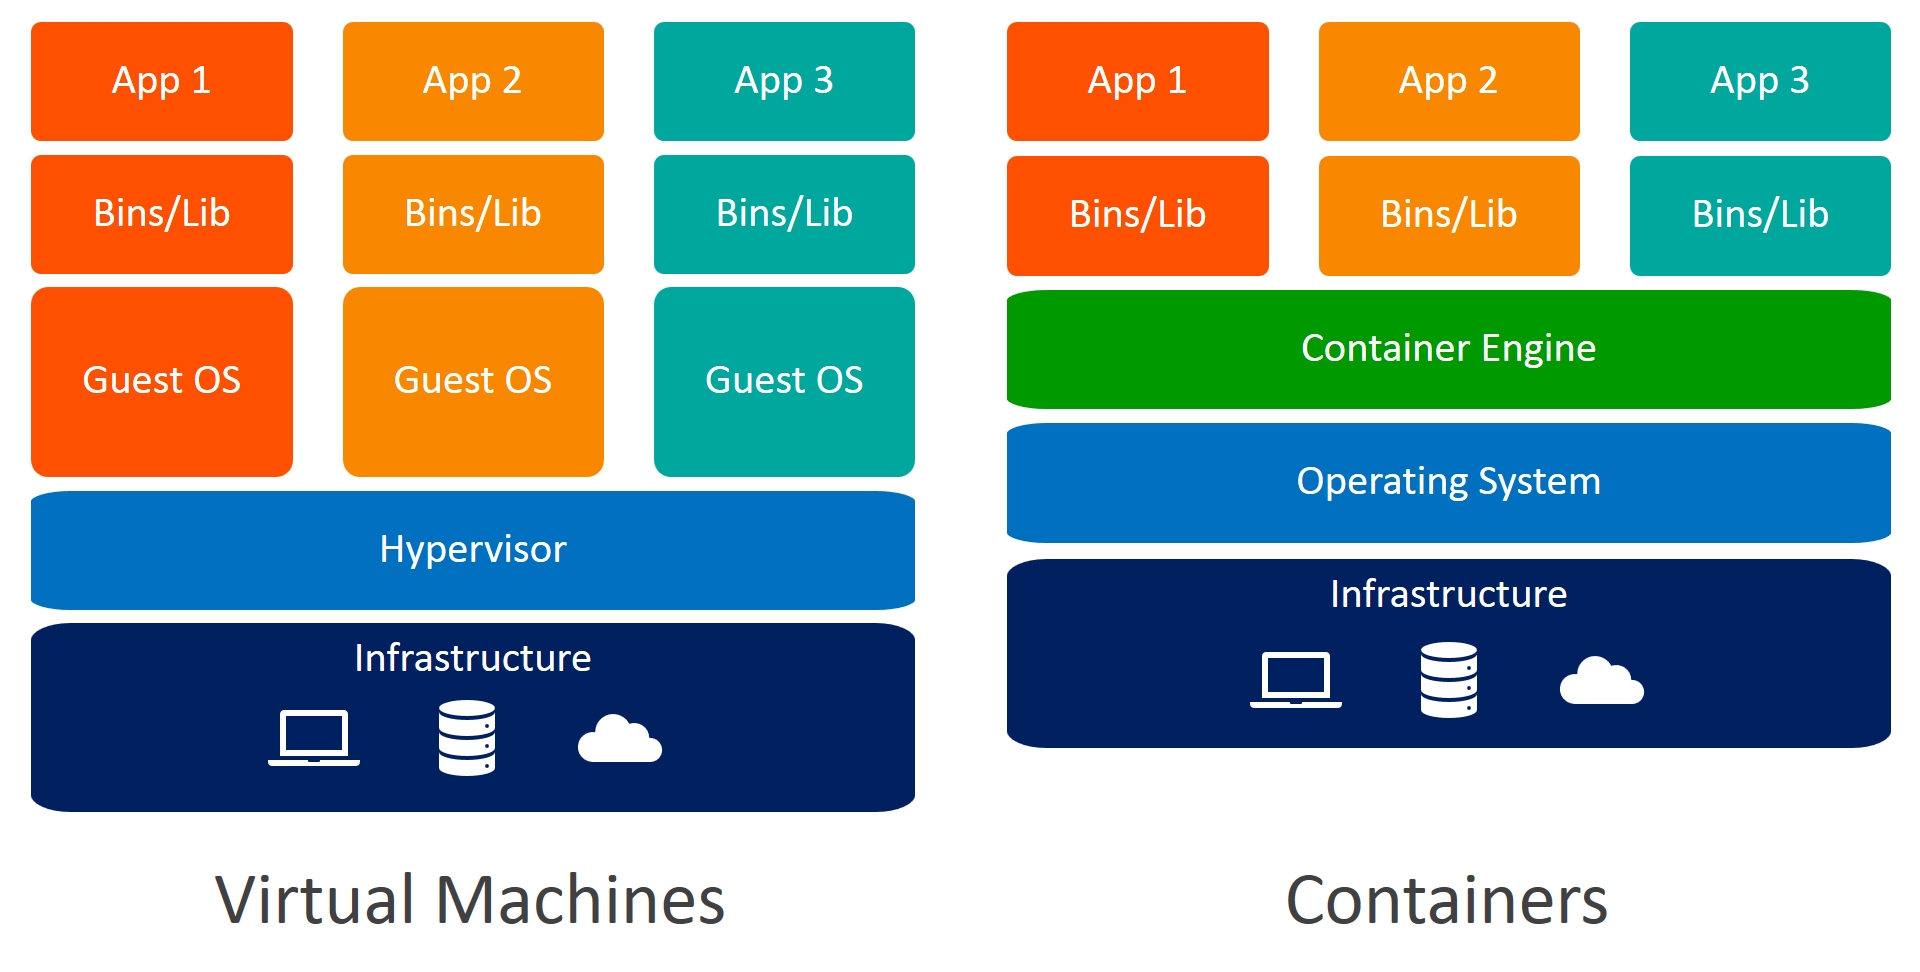
\includegraphics[width=.9\textwidth]{figures/containervsvirtual}
    \caption{\ Porovnanie infraštruktúry kontajnera a virtualizácie \cite{containervsvirtual} \label{o:latex_friendly_zone}}
\end{figure}

\subsection{Systemový a aplikačný kontajner}

Aplikačné kontajnery, ako napríklad Docker, zapuzdrujú súbory a knižnice aplikácie, ktoré sa majú spustiť na operačnom systéme. Aplikačné kontajnery umožňujú používateľovi vytvoriť a spustiť samostatný kontajner pre viacero nezávislých aplikácií alebo viacero služieb, ktoré tvoria jednu aplikáciu. Napríklad aplikačný kontajner by bol vhodný pre aplikáciu mikroslužieb, kde každá služba, ktorá tvorí aplikáciu, beží nezávisle jedna od druhej.

Systémové kontajnery, sú technologicky podobné kontajnerom aplikácií aj virtuálnym strojom. Systémový kontajner môže spúšťať operačný systém, podobne ako by operačný systém bežal zapuzdrený na VM. Systémové kontajnery však neemulujú hardvér systému, namiesto toho fungujú podobne ako aplikačné kontajnery a používateľ si môže nainštalovať rôzne knižnice, jazyky a systémové databázy. \cite{systemvsapli}

Takže všeobecne, keď chcete distribuovať aplikáciu ako komponenty, aplikačné kontajnery sú skvela voľba. Zatiaľ čo ak chcete iba operačný systém, do ktorého môžete nainštalovať rôzne knižnice, jazyky, databázy atď. vhodnejšie sú systémové kontajnery.


\clearpage
\begin{itemize}
    \item v~knihe \cite{book} autor prezentuje naozaj odvážne myšlienky
    \item nemenej zaujímavé výsledky publikuje ďalší autor v~článku \cite{article} 
    \item v~konferenčnom príspevku \cite{conference} sú uvedené tiež zaujímavé veci
    \item \LaTeX{}\footnote{\url{https://www.latex-project.org/}} je typografický jazyk
\end{itemize}

Given a set of numbers, there are elementary methods to compute its \acrlong{gcd}, which is abbreviated \acrshort{gcd}. This process is similar to that used for the \acrfull{lcm}.

\subsection{Donec vehicula consequat}
\blindtext



\subsection{Nullam in mauris consectetur}
\blindtext

\begin{lstlisting}[language=C,caption={Program, ktorý pozdraví celý svet}]
#include <stdio.h>
int main() {
    /* Print Hello, World! */
    printf("Hello, World!\n");
    return 0;
}
\end{lstlisting}


\subsection{Vestibulum tristique elementum varius}
\blindtext

\begin{table}[!ht]
	\caption{Country list}\label{t:1}
	\smallskip
	\centering

	\begin{tabular}{ |p{3cm}||p{3cm}|p{3cm}|p{3cm}|  }
		\hline
		\multicolumn{4}{|c|}{Country List} \\
		\hline
		Country Name or Area Name& ISO ALPHA 2 Code &ISO ALPHA 3 Code&ISO numeric Code\\
		\hline
		Afghanistan & AF & AFG & 004\\
		Aland Islands & AX & ALA & 248\\
		Albania & AL & ALB & 008\\
		Algeria & DZ & DZA & 012\\
		American Samoa & AS & ASM & 016\\
		Andorra & AD & AND & 020\\
		Angola & AO & AGO & 024\\
		\hline
	\end{tabular}
\end{table}


\section{Phasellus id pretium neque}
\blindtext

\blindtext

% !TEX root = ../thesis.tex

\chapter{Využitie technologií v praxi}
\label{methodology}

Na vyriešenie problematiky nasadenia strojového učenia na platforme Kubernetes sú v tejto časti poskytnuté postupy na lokálne nasadenie na zariadeniach ako je laptop alebo stolný počítač. Jedna sa prevažne o platformu Kubeflow. Riešenia, ktoré sú poskytnuté sú mierne hardverovo záťažové, čo znamená, že sú vhodné pre zariadenia s hardvérovým vybavením minimálne 2 GB veľkou operačnou pamäťou a s voľným priestorom na disku. Dodané postupy sú vhodné, či už pre slabšie zariadenia ale aj výkonovo silnejšie pre plné nasadenie platformy.

\section{Kubeflow}
Kubeflow ako platforma, je vhodná na nasadenie a vývoj strojového učenia. Primárne slúži pre inžinierov a vedcov, ktorý pracujú s dátami. Obsahuje viaceré komponenty, z ktorých si vývojári môžu vybrať, čo je pre ich používateľov najlepšie, čo znamená, že na nasadzovanie nie je potrebný každý jeden komponent.

\subsection{Komponenty}

Stavia na platforme Kubernetes ako systéme na nasadenie, škálovanie a správu zložitých systémov. Pomocou konfiguračných rozhraní Kubeflow, môžeme špecifikovať nástroje strojového učenia, potrebné pre náš pracovný postup. Potom môžeme nasadiť pracovný postup do rôznych cloudov, miestnych platforiem na experimentovanie a na produkčné použitie.

V tejto časti sú priblížené všetky šesť komponenty, ktoré tvoria Kubeflow.


\subsection*{Pipelines}

Pipelines sa používajú na vytváranie a nasadzovanie prenosných, škálovateľných, pracovných postupov strojového učenia založených na kontajneroch Docker. Pozostávajú z používateľského rozhrania na správu tréningových experimentov, úloh a chodov a z nástroja na plánovanie viackrokových pracovných postupov strojového učenia. Existujú aj dve súpravy SDK, jedna umožňuje definovať a manipulovať s pipelines, zatiaľ čo druhá ponúka alternatívny spôsob interakcie Notebookov so systémom \cite{pipe}.

\subsection*{Notebooks}

Jupyter notebooks fungujú s Kubeflow veľmi dobre, pretože sa dajú ľahko integrovať s typickými mechanizmami overovania a kontroly prístupu. Používatelia môžu bezpečne a s istotou vytvárať notebookové moduly/servery priamo v klastri Kubeflow pomocou obrazov poskytnutých správcami a jednoducho odosielať úlohy s jedným uzlom v porovnaní s tým, že si musia všetko nakonfigurovať na svojom laptope.


\subsection*{Katib}

Katib je škálovateľný a rozšíriteľný framework, ktorý podporuje ladenie hyperparametrov a vyhľadávanie neurónovej architektúry. Umožňuje používateľom objaviť modely, ktoré sú rovnako dobré ako ručne vytvorené modely, bez toho, aby museli prejsť namáhavým manuálnym procesom konfigurácie a opakovania. Katib organizuje optimalizáciu alebo vyhľadávanie neurónovej architektúry a presúva ju do sekcie s názvom Experiment. Algoritmy bežia interaktívnym spôsobom. Experiment definuje vyhľadávací priestor, cieľ metrík a maximálny počet iterácií. Katib hľadá iteratívne vo vyhľadávacom priestore, aby splnil cieľ metrík alebo aby dosiahol maximálny počet opakovaní. Katib podporuje dva rôzne mechanizmy – Hyperparameter Tuning a Neural Architecture Search \cite{katib}.

Ladenie hyperparametrov je proces optimalizácie hodnôt hyperparametrov modelu s cieľom maximalizovať predikčnú kvalitu modelu. Príkladmi takýchto hyperparametrov sú rýchlosť učenia, hĺbka neurálnej architektúry (vrstvy) a šírka (uzly), epochy, veľkosť dávky, miera výpadkov a aktivačné funkcie. Toto sú parametre, ktoré sa nastavujú pred tréningom; na rozdiel od parametrov modelu (váhy a odchýlky) sa tieto nemenia počas procesu trénovania modelu.

\subsection*{Training operators}

Operátor Kubeflow pomáha nasadzovať, monitorovať a spravovať životný cyklus Kubeflow. Je zložený z Operator frameworku, čo je súprava nástrojov s otvoreným zdrojovým kódom na zostavovanie, testovanie, balenie operátorov a správu životného cyklu operátorov. Operátor Kubeflow používa KfDef ako svoj vlastný zdroj a kfctl ako základný nástroj na spustenie operátora.

Napríklad operátor k8s spadá pod Kubeflow. Tento operátor uľahčuje spúšťanie úloh tensorflow, či už sú distribuované alebo nedistribuované na kubernetes. TFjobs sú vlastným zdrojom Kubernetes, ktorý sa používa na trénovanie alebo spustenie úloh trénovania na Kubernetes. Kubeflow udržiava všetky tieto operátory a dá sa povedať, že Kubeflow zhromažďuje také komponenty, ktoré uľahčujú spustenie kódu strojového učenia v rôznych formách v rámci Kubernetes. Takže potrebný je operátor pre TFJob, ktorý to bude monitorovať a sledovať. Nasadenie Kubeflow, dokáže rozšíriť nasadenia operátorov, a potom podľa toho definovať TFjobs a spustiť toľko, koľko tréningov je potrebné na klastri kubernetes \cite{operator}.

\subsection*{Multi-Tenancy}

Po nainštalovaní a nakonfigurovaní Kubeflow sa predvolene pristupuje k primárnemu profilu. Profil vlastní menný priestor Kubernetes s rovnakým názvom spolu s kolekciou zdrojov Kubernetes. Používatelia majú prístup na zobrazenie a úpravu svojich primárnych profilov. Prístup k profilu je možné zdieľať s iným používateľom v systéme. Pri zdieľaní prístupu k profilu je na výber, aký prístup je možné poskytnúť na čítanie alebo prístup na čítanie/úpravu. Na všetky praktické účely pri práci s centrálnym ovládacím panelom Kubeflow je aktívny menný priestor priamo prepojený s aktívnym profilom.

\subsection*{Rozhranie}

Centrum riadenia komponentov, ktoré poskytuje používateľovi prístup k jednotlivým komponentom v klastri ako sú Pipelines, Notebooks, Katib, Artifact store a Multi-Tenancy.

Na nasledujúcom obrázku je možné vidieť rozhranie a niektoré komponenty, ktoré kubeflow ponúka.

\clearpage

\begin{figure}[h!]
    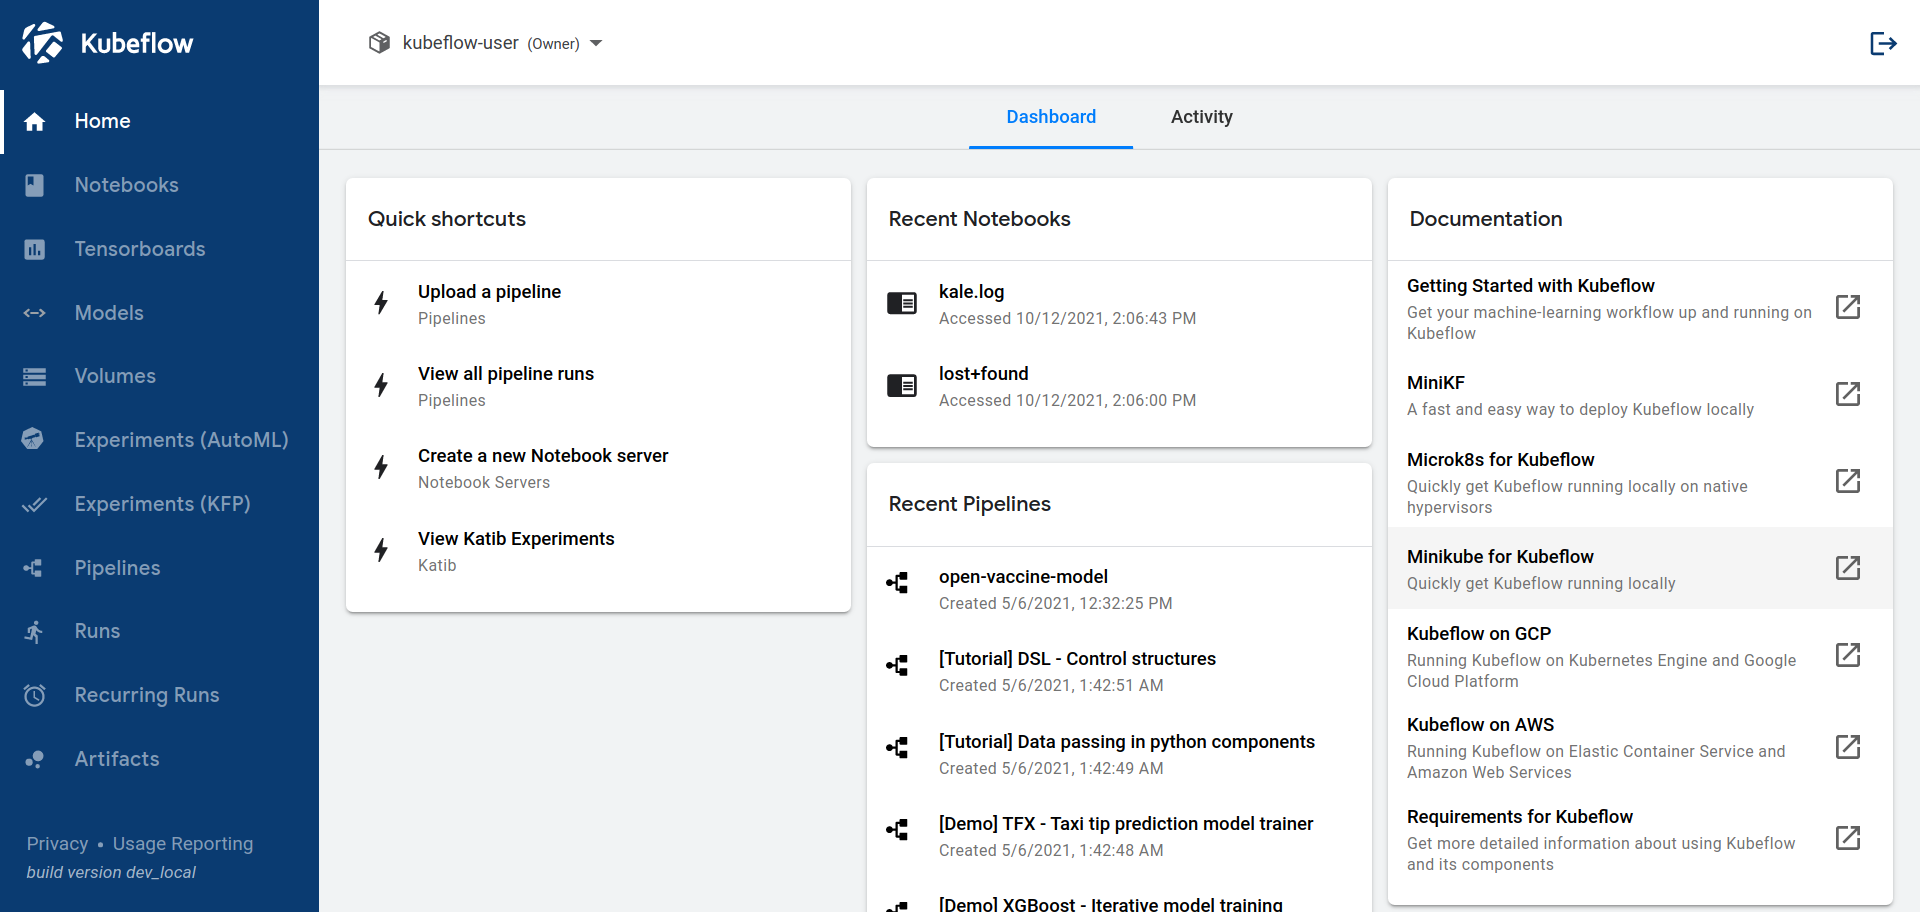
\includegraphics[width=\linewidth]{figures/Rozhranie}
    \caption{ Rozhranie Kubeflow }
\end{figure}

\subsection{Pracovný postup}

Postup pozostáva z viacerých krokov, taktiež z iterácie, ktorá je hlavným prvkom pri vyvíjaní sýtemu strojového učenia. Pri tomto postupe je potrebné vykonávať zmeny v parametroch aby sme dosiahli požadované výsledky. Následne si povieme niečo viac o týchto postupoch.

Ako prvé by sme mali vyvíjať model na základe predpokladov a testov. Môžeme ho opísať v nasledujúcich bodoch: \cite{work}

\begin{itemize}
    \item Identifikovanie problému, ktorý ma systém vyriešiť.
    \item Zbieranie dát, ktoré potrebujeme na trénovanie modelu.
    \item Vyberanie algoritmu a nakódovanie modelu.
    \item Experiment s údajmi a trénovanie modelu.
	\item Vyladenie parametrov.
\end{itemize}

Ďalej môžeme nasadiť systém, ktorý bude vykonávať tieto procesy:

\begin{itemize}
    \item Transformáciu údajov, ktoré náš systém potrebuje.
	\item Trénovanie modelu.
	\item Podanie modelu na online prevádzku.
	\item Monitorovanie výsledkov na úpravu a zmenu modelu.
\end{itemize}

\begin{figure}[!ht]
    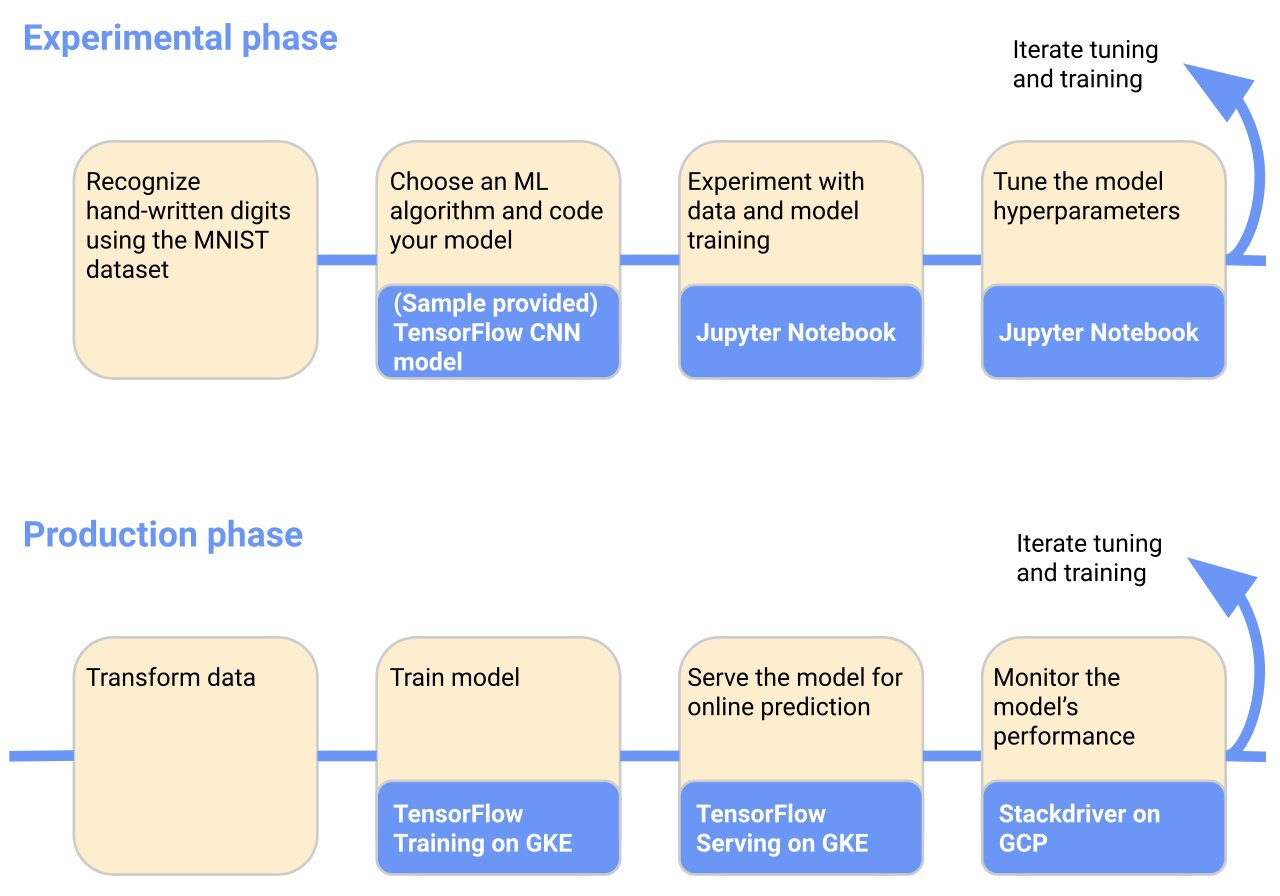
\includegraphics[width=.9\textwidth]{figures/kubeflowwork}
    \caption{\ Pracovné postupy \cite{work} \label{o:latex_friendly_zone}}
\end{figure}

\section{MiniKF}

Je softvér, vyvinutý spoločnosťou Arrikto, a to kombináciou viacerých služieb a nástrojov potrebných na spustenie úloh strojového učenia lokálne alebo vzdialene na platforme Kubernetes. Skladá sa z nástroja minikube na spustenie lokálnej platformy Kubernetes, samotného Kubeflow a platformy Rok, ktorá umožňuje spúšťanie stavových kontajnerov cez rýchle lokálne úložisko NVMe. MiniKF je lokálne nasadenie Kubeflow, ktoré je možné nainštalovať v priebehu minút. Po niekoľkých kliknutiach je možné začať experimentovať a dokonca spúšťať Machine Learning Pipelines.

Pred inštaláciou je potrebné nainštalovať VirtualBox a Vagrant. Je to softvér na vytváranie a udržovanie prenosných prostredí. Pre lokálne spustenie MiniKF je potrebné spĺňať minimálne požiadavky pre operačnú pamäť minimálne 12 GB, 2 jadra procesora a 50 GB voľného miesta na disku. Na operačnom systéme nezáleží, pretože je ho možné virtualizovať na rôznych operačných systémoch napríklad ako je Linux, macOS a Windows.

Inštalácia prebieha jednoducho a pozostáva z dvoch príkazov. Prvým príkazom sa stiahne konfiguračný súbor alebo obraz do daného priečinka a inicializujeme virtuálny počítač.
\begin{lstlisting}[language=Bash]
    $ vagrant init arrikto/minikf
    \end{lstlisting}
Druhým príkazom sa zapne virtuálny počítač a spustí sa konfiguračný súbor.
\begin{lstlisting}[language=Bash]
    $ vagrant up
    \end{lstlisting}
Kubeflow je poháňaný prostredníctvom Kubernetes na tomto virtuálnom počítací. Ak je virtuálny počítač pripravený spusti sa na ňom skript a následne je možné sa pripojiť cez internetový prehliadač na adrese 10.10.10.10 k danému počítaču, kde sa spustí nástroj, ktorý developuje serie softvérových balíčkov potrebných na spustenie Kubeflow. Po reštartovaní počítača sa dáta nestratia, stačí zopakovať postup a je možné sa vrátiť k začatej práci.

\section{Charmed}

Pri developovaní Kubeflow sa pri tomto spôsobe využíva Juju Charm. Juju Charm je bezplatný aplikačný nástroj na modelovanie aplikácii s otvoreným zdrojovým kódom vyvinutý spoločnosťou Canonical, je známy aj ako štruktúrovaný balík konfiguračných súborov YAML a skriptov pre softvérový komponent, ktorý umožňuje Juju nasadiť a spravovať softvérový komponent ako službu podľa osvedčených postupov. Poskytuje centrálny pohľad na operátorov Kubernetes v nasadení, konfigurácií, rozsahu a stavu každého z nich a integračných liniek medzi nimi. Sleduje potenciálne aktualizácie a inovácie pre každého operátora a koordinuje tok udalostí a správ medzi operátormi.

Tento spôsob je vhodný najmä pre používateľov s operačným systémom Ubuntu. Samozrejme ho je možné použiť aj na iných operačných systémoch použitím virtualizácie, odporúča sa využiť Multipass, nenáročného správcu virtuálnych počítačov Ubuntu. Poskytuje virtualizáciu využitím Hyper-V alebo VirtualBoxu. Minimálne požiadavky závisia od verzie Kubeflow a to pri verzii full sú väčšie, minimálne 16 GB operačnej pamäte a 60 GB voľného miesta na disku. Full verzia poskytuje všetky služby napríklad Katib a Jupyter Notebooks. Verzia s označením lite bola vytvorená pre používateľov, ktorí pracujú v prostredí s obmedzenými zdrojmi a mal by fungovať dobre pri 8 GB operačnej pamäte a 50 GB dostupných na disku. Zachováva užívateľsky dashboard, ktorý je vhodný najmä pre začiatočníkov s lepšou interakciou. Tento balík je orientovaný najmä na nasadenie na systémoch ako notebook. Poslednou a najľahšou verziou je edge, ktorá neobsahuje dashboard a je vhodná pre tých, ktorí vyžadujú vlastných operátorov alebo pre zariadenia so slabšími výkonom. Na spustenie postačuje 4 GB operačnej pamäte. Pri každej verzii sú potrebné 4 jadra procesora. Je možné tieto verzie aj editovať, ak neobsahujú niečo potrebné a to upravením YAML súboru.

Prvým krokom je nainštalovať Multipass, ak postup sa vykonáva na zariadení, ktorý ma operačný systém iný ako Ubuntu. Pre správne fungovanie sa využíva MicroK8s pre spravovanie klastra s 1.21 verziou Kubernetes. Je dostupná aj novšia verzia s označením 1.22, ktorá zatiaľ nepodporuje Kubeflow. Aby ďalšie príkazy fungovali bez použitia sudo je treba pridať používateľa do skupiny. Ak je Kubernetes pripravený, dostupné sú viaceré služby. Aby sa navzájom našli aplikácie, úložisko, prístup ku komponentom Kubeflow a aplikácii na vyrovnávanie záťaže MetalLB je nutné pridať DNS službu. Pred ďalšími krokmi sa kontroluje, či boli služby povolené. Pre developovanie Kubeflow platformy je nevyhnutný Juju nastroj. Jeho inštalácia je pomerne jednoduchá, pretože sa inštaluje z balíka využitím systému snap na spravovanie balíčkov. Spustenie príkazu na nasadenie ovládača Juju do Kubernetes pre ovládanie komponentov Kubeflow a odporúča sa taktiež nastaviť špecificky model. Po Juju nasleduje proces nasadenia Kubeflow a je treba vyčkať pokiaľ sa jednotlivé aplikácie a komponenty pripravia a budú môcť medzi sebou komunikovať. Pre prístup k dashboardu nakonfigurovanie niektorých komponentov je nevyhnutné s povolenou adresou URL. K dispozícii je aj možnosť nastavenia mena a hesla. Na záver je možné zobraziť dashboard v prehliadači s URL, ktorú sme nakonfigurovali. Ak sa využíva Multipass pre získanie prístupu je vhodné vytvoriť pripojenie použitím SSH so zapnutým SOCKS proxy.

\subsection{Pripojenie strojov do klastra}

Pridanie viacero uzlov (strojov) do klastra Kubernetes znamená, že pracovné zaťaženie môže byť rozdelené medzi rôzne uzly, ktoré sa môžu škálovať podľa ich špecifického zaťaženia. Nasadenia viacerých klastrov sú rozdelené do viacerých uzlov a škálujú sa podľa zaťaženia konkrétneho klastra. Čím drasticky znižuje spotrebu zdrojov jedného uzla a vedie k menšiemu zaťaženiu backendových služieb, ako sú databázy. Na rozdiel od modelu s jedným klastrom, prevádzkovanie v pracovných zaťažení poskytuje tvrdú úroveň izolácie. Riziko vzájomnej interakcie aplikácií alebo aplikácií s viacerými prostrediami, neúmyselným spôsobom je výrazne nižšie. Poskytuje lepši výkon poprepájaním strojov, ktorý je veľmi dôležitý pri strojovom učení. V tomto prípade je podstatnejší viacuzlový klaster než jednouzlový, najmä kvôli tomu, ak niektorý z hlavných uzlov zlyhá, ostatné uzly udržia klaster v prevádzke. Preto je vhodné vytvorenie viacuzlového klastra pripojením ďalších uzlov.

Postup je odlišný len na základe operačných systémov v ktorých sa bude pripájanie vykonávať. Požiadavky podľa oficiálnej dokumentácie sú nasledovné:

\begin{itemize}
    \item Každý uzol v klastri by mal mať aspoň 2GB pamäte RAM a 2 jadra procesora.
    \item Samozrejmosťou je verejné alebo súkromné sieťové pripojenie pre všetky stroje v klastri.
    \item Názov hostiteľa a MAC adresa musia byť jedinečné.
    \item Funkcia swap space, ktorá slúži na rozšírenie RAM pamäte na linuxových distribúciách musí byť vypnutá.
    \item Každý uzol vyžaduje svoje vlastné plne izolované prostredie - samostatný fyzický počítač, virtuálny stroj, kontajner alebo iný počítač v rovnakej sieti. V jednom prostredí nie je možné spustiť dve pracovné inštancie.
\end{itemize}

\subsection*{Linux/Ubuntu}

Ako prvé je potrebné spustiť tento príkaz na počítací, ktorý chceme aby bol riadiacim klastrom a zároveň hostiteľom riadiacej roviny Kubernetes.

\begin{lstlisting}[language=Bash]
    $ microk8s add-node
    \end{lstlisting}

Príkaz vygeneruje link s pokynmi na dočasnú registráciu pre nový uzol. V pokynoch sú príkazy, ktorými je možne vykonať spojenie uzla s riadiacou rovinou. Jeden z týchto príkazov sa spúšťa na stroji, ktorý chceme spojiť s uzlom, na ktorom bol spustení predošli príkaz. Proces pripojenia trvá niekoľko sekúnd. Pokyny su názorne ukázané na nasledujúcom obrázku.

\begin{figure}[h!]
    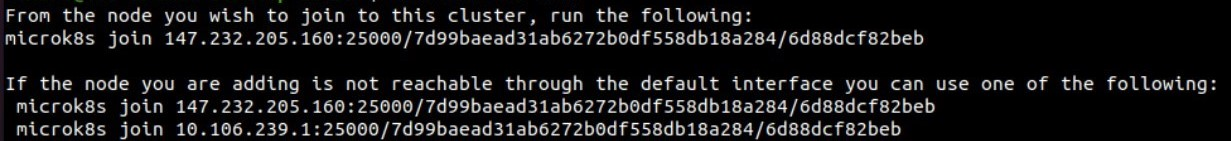
\includegraphics[width=\linewidth]{figures/addnode}
    \caption{ Príkazy na pripojenie stroja do klastra }
\end{figure}

Po pridaní uzla je možné hostiť pody na viacerých strojoch. Všetky dostupné uzly sa zobrazujú spustením príkazu:

\begin{lstlisting}[language=Bash]
    $ microk8s kubectl get nodes
    \end{lstlisting}

\subsection*{Windows Server 2019 alebo novší}

Pre zlúčenie stroja s operačným systémom Windows je dôležitý Docker na správu kontajnerov a pripravený klaster s Calico CNI. Je to sieťovo kontajnerové rozhranie označované ako CNI, ktoré rieši množstvo sieťových požiadaviek napríklad komunikáciu medzi kontajnermi alebo externými službami. Zároveň sa vyžaduje aj inštalácia calicoctl, nástroj príkazového riadka pre spravovanie Calico a vykonávanie administratívnych funkcii.

Pre prístup do klastra sa vyžaduje kópia súboru kubeconfig. Pre pody na Windowse musí byť strictaffinity nastavená na hodnotu ako pravdivá, aby sa zabránilo požičiavaniu IP adries z uzlov Windowsu. Vhodné je sa ubezpečiť aká verzia Kubernetes je nasadená v klastri.

Ďalším krokom je inštalácia komponentov na stroji s operačným systémom Windows pomocou prostredia PowerShell spustený ako správca. Inštalácia pozostáva z vytvorenia priečinka, do ktorého uložíme predošlú kópiu súboru kubeconfig, inštalácie systému Calico a spustenia služby Kubernetes.

\subsection{Odpojenie stroja z klastra}

Zmazanie stroja z klastra je jednoduché a uskutočňuje sa pomocou dvoch príkazov. Príkazy sa použijú na stroji, ktorý ma byť odstránení z klastra.

Microk8s reštartuje riadiacu rovinu na uzle, ktorý sa ma vymazať. Tým obnoví operácie a stane sa osobitným klastrom. V pôvodnom klastri sa označí ako nedostupný a nebudú sa naň nasadávať nove operácie.
\begin{lstlisting}[language=Bash]
    $ microk8s leave
    \end{lstlisting}
Pre úplne vymazanie stroja zo zostávajúcich uzlov sa používa nasledujúci príkaz s jeho IP adresou:
\begin{lstlisting}[language=Bash]
    $ microk8s remove-node <node_IP>
    \end{lstlisting}
\subsection{Podpora grafickej karty}

Implementovanie grafickej karty do klastra Kubernetes je veľkou výhodou najmä kvôli výraznému skráteniu času na riešenie náročno výpočtových operácií. Je veľkou výhodou pri strojovom učení. Pridanie grafickej karty vykonáme prostredníctvom tohto príkazu.

\begin{lstlisting}[language=Bash]
    $ microk8s enable gpu
    \end{lstlisting}

Pre pridanie grafickej karty je potrebné splniť nasledujúce body:

\begin{itemize}
    \item Platforma Kubeflow verzia full alebo lite je spustená v Kubernetes klastri.
    \item Je dostupné pripojenie na internet.
    \item Bolo uskutočnené prihlásenie prostredníctvom Kubeflow dashboardu.
    \item V hardvérovom vybavení je dostupná grafická karta od spoločnosti AMD alebo NVIDIA.
\end{itemize}

Ak je grafická karta povolená a pridaná do klastra niektoré pracovné úlohy môžu ju požadovať nastavenim limitu napríklad ako nvidia.com/gpu: 1.

\subsection{High aviability}

\section{Pipelines}

Tento spôsob je vhodný, vtedy ak je žiadaná práca výhradne s Kubeflow pipelines. Cieľom je nasadiť pipelines na lokálnom klastri. Na nasadenie nie sú nutné žiadne virtualizačné programy a postup je v celku jednoduchý, pretože sú tým výnimočne. Kubeflow pipelines sú známe kontajnerizáciou, čo znamená, že bude sa používať Docker na vytváranie kontajnerov. Požiadavky na spustenie nie sú náročne, pre operačnú pamäť si vyžadujú minimálne 8 GB a 2 jadra procesora. Nástroj kind je kľúčový, slúži na vytvorenie lokálneho Kubernetes klastra využitím Dockera. Taktiež by bolo dobre poznamenať, že Docker vyžaduje Windows Subsystem for Linux (WSL), ktorý slúži pre natívny beh linuxových spustiteľných súborov v prostredí Windows. Pre správny postup inštalácie sa požaduje aj kubectl, ktorý sa používa na komunikáciu s klastrom vyžitím príkazového riadka a Git.

Na začiatok je potrebné nainštalovať nástroj kind. Inštalácia na operačnom systéme Windows je veľmi jednoduchá a pozostáva z niekoľko príkazov, pripadne je možné použiť Chocolatey, ktorý je vhodný na inštaláciu balíčkov na systéme Windows. Ďalším krokom je vytvorenie klastra príkazom “kind create cluster”.  Kind spusti klaster Kubernetes pomocou vopred vytvoreného obrazu. Samozrejmosťou je použitie vlastného obrazu. Nasadenie pipelines sa vykoná spustením príkazov, ktoré stiahnu všetko potrebné z gitu a treba počkať niekoľko minút pokiaľ prebehne nasadenie všetkých komponentov potrebných pre pipelines a následne posledným krokom je presmerovanie portov. Po presmerovaní je Kubeflow dostupný otvorením internetového prehliadača na adrese „http://localhost:8080/“.

\section{Kubeadm}

Pri tomto postupe sa využíva nástroj Kubeadm, ktorý bol zavedený pre vytváranie Kubernetes klastrov. Je vyvíjaný oficiálnou komunitou Kubernetes. Poskytuje minimalisticky systém, veľmi dobru portabilitu a lokálne nasadenie na strojoch, ako sú napríklad notebook, Raspberry PI a podobne. Znižuje zložitosť a uľahčuje nasadenie použiteľného klastra Kubernetes. Minimálne požiadavky pre funkčný beh Kubernetes sú 2 GB operačnej pamäte a dve jadra procesora pre jeden stroj. V prípade riešeného problému tejto bakalárskej práce sa vyžaduje kvôli nasadeniu Kubeflow viac zdrojov. Záleží to od faktorov ako počet komponentov, ktoré sú požadované, koľko strojov je pripojených v klastri a s akými zdrojmi. Pre vytváranie kontajnerov nasadenie pozostáva aj z inštalácie vhodnej kontajnerovej služby ako je Docker.

Inštalácia je vykonávaná na linuxovej distribúcii. Pred nastavením klastra prostredníctvom Kubeadm je potrebné povoliť prenos cez firewall prostredníctvom IPtables. Funkcia Swap je aj v tomto spôsobe zakázaná. Základnou požiadavkou je nejaký obraz kontajnera. Na výber sú viaceré služby ako containerd, CRI-O alebo Docker. Po úspešnom nastavení je dôležité povoliť služby využívajúce kontajnerizáciu v systéme. Nutné je konfigurovať Kubeadm, Kubelet a Kubectl na verziu 1.21, keďže Kubeflow je do tejto verzie podporovaný a musí sa striktne dodržať. Pre prevenciu, aby sa programy neaktualizovali sa musia označiť ako hold, čo zabraní samovoľnému aktualizovaniu na novšiu verziu. Nasleduje inicializácia klastra na počítací prostredníctvom Kubeadm, ktorý bude riadiacou rovinou v platforme Kubernetes. Po úspešnej inicializácii Kubeadm sa vypíše výstup s umiestnením súboru kubeconfig, ktorý využíva Kubectl na interakciu s klastrom a príkaz join s tokenom. Je dobré ho niekde uchovať alebo neskôr znova vypísať, pretože je potrebný pri pridávaní stroja. V predvolenom nastavení sa pody nenaplánujú na hlavnom uzle. Hlavný uzol sa môže použiť na nasadzovanie podov, ak sa označí ako pracovný uzol. Kubeadm nenakonfiguruje žiadny sieťový doplnok. Pre správne fungovanie sa nastavuje sieťový doplnok ako Calico.

Ak je všetko dobre nastavené, overiť sa to da prostredníctvom príkazu Kubectl na vypísanie počítačov v klastri, či je daný poctiac pripravený. Počítač musí byť v stave Ready, čo znamená, že je pripravený na ďalšie kroky nasadzovania. Vhodné je aj nasadenie UI dashboardu pre lepšiu interakciu používateľa s platformou.

Spustenie Kubeflow platformy sa realizuje manuálnou inštaláciou manifestov. Existujú aj rôzni distribútori ako Google, Amazon alebo IBM. Ich služby a ich realizácia je jednoduchšia, sú však spoplatnené. Kubeflow vyžaduje nastavenie Kubernetes s prednastaveným StorageClass a nástroja Kustomize, ktorý slúži na prispôsobovanie objektov pomocou jeho Kustomize súborov. Kubeflow s verziou 1.5 zatiaľ nie je kompatibilný s najnovšou verziou Kustomize, preto musí byť verzia 3.2. Do počítača si naklonujeme oficiálny git repozitár od spoločnosti Kubeflow. Sú dva spôsoby implementovania manifestov použitím jedného, kde sa použijú všetky existujúce komponenty alebo pomocou viacerých príkazov a to vlastným výberom komponentov, ktoré sa vyžadujú. Po niekoľkých minútach sú všetky komponenty pripravené. A posledným krokom ostáva zapnutie Dashboardu, kde používateľ môže naplno využívať komponenty.

\subsection{Pripojenie strojov do klastra}

Implementácia a požiadavky sú podobné ako pri predchádzajúcom pripájaní strojov do klastra využitím Charmed Kubeflow nasadenia.

\subsection*{Linux/Ubuntu}

Pre pripojenie linuxového stroja je nutné na ňom zopakovať niektoré inštalačné postupy, ktoré boli vykonané pri konfigurácii Kubernetes klastra:

\begin{itemize}
    \item Povolit prenos cez Firewall pomocou IPtables
    \item Zákaz funkcie Swap
    \item Docker
    \item Kubeadm, Kubelet, kubectl
\end{itemize}

Po týchto krokoch je možné použiť hore spomínaný príkaz join na pripojenie stroja do klastra.

\subsection*{Windows Server 2019 alebo novší}

Spustenie a spojazdnenie komponentov pre platformu Kubernetes na Windowse je obťažnejšie a môže byt problémové. Pre pridanie stroja s operačným systémom Windows do klastra, ktorý beží na Linuxe je na ňom treba vykonať doplnkové akcie.

Na stroji, ktorý nesie označenie hlavnej roviny sa stiahne Flannel manifest, v~ktorom sa upravia čísla portov, aby Linux spolupracoval s Flannelom v systéme Windows. Flannel sa používa na priraďovanie IP adries kontajnerom a pre komunikáciu medzi nimi. Editovanú konfiguráciu je možné aplikovať do klastra. Treba však aj tu poznamenať dodržanie verzii, aby súladili s verziou Kubernetes spustenej na klastri. Po chvíli sa vytvoria sieťové Flannelové moduly.

Na stroji s Windowsom, ktorý sa pridáva do klastra vykonáme inštaláciu Dockera s verziou Engine Enterprise a povolenie funkcie Hyper-V. Na rade sú Wins, Kubelet a Kubeadm, ktoré musia mať rovnakú verziu ako klaster Kubernetes. Ako posledná akcia, ktorá by sa mala vykonať je použitie príkazu join.

\subsection{Odpojenie stroja z klastra}

Odstránenie prebieha pomocou nástroja kubectl, použitím nasledovných príkazov na riadiacej rovine.

Označenie stroja ako neplánovateľný, aby sa zamedzilo pridávaniu nových podov.

\begin{lstlisting}[language=Bash]
    $ kubectl cordon <node_ID>
    \end{lstlisting}

Bezpečné odstránenie všetkých podov z uzla pred odstránením. Vysťahovanie kontajnerov, aby sa mohli ukončiť pody na stroji, ktorý sa odstraňuje. Ak všetko prebehne v poriadku, znamená to, že všetky pody boli bezpečne odstránené alebo presunuté.

\begin{lstlisting}[language=Bash]
    $ kubectl drain <node_ID>
    \end{lstlisting}

Následne je možné prejsť k odstráneniu všetkých údajov o danom stroji z klastra.

\begin{lstlisting}[language=Bash]
    $ kubectl delete node cmp<node_ID>
    \end{lstlisting}

\subsection{Podpora grafickej karty}

Pridanie grafickej karty sa sprostredkuje prostredníctvom grafických kariet od spoločnosti NVDIA a AMD. Podmienkou je mať nainštalované ovládače od grafických kariet.
Operácia aplikovania grafickej karty je vykonaná prostredníctvom príkazu s manifestom vo forme YAML súboru podľa toho o akú grafickú kartu ide.

\begin{lstlisting}[language=Bash]
    $ kubectl create -f <manifest>
    \end{lstlisting}

Ak sa jedná o grafickú kartu spoločnosti NVIDIA je nutné spraviť dodatočné opatrenia:

\begin{itemize}
    \item Vopred nainštalovaný nástroj pre kontajnery nvidia-docker s verziou 2.0.
    \item Kubelet musí používať Docker ako svoj kontajnerový obraz.
    \item Nvidia-container-runtime nakonfigurovaný ako predvolený runtime pre Docker namiesto runc.
\end{itemize}

% !TEX root = ../thesis.tex

\chapter{Výsledky testovania technologií}
\label{evaluation}

V tejto kapitole je zhrnuté porovnanie testovaných scenárov a postupov na nasadenie platformy Kubernetes a Kubeflow, ktoré sa využívajú na riešenie problémov strojového učenia. Priblížené sú problémy, ktoré sa vyskytovali pri uplatňovaní týchto plánov, ich zvládnutie, objektívne vyhodnotenie týchto technológii a vyzdvihnutie najlepšieho spôsobu.

Testovanie prebiehalo na serveroch od portálu CLOUD TUKE s operačnými systémami Windows server 2019 a Ubuntu 20.04 Desktop s nasledovnými parametrami:

\begin{itemize}
	\item Procesor: \textbf{Intel(R) Xeon(R) CPU E5-2670 v3 @ 2.30GHz}
	\item Počet jadier: \textbf{8}
    \item Veľkosť operačnej pamäte RAM: \textbf{16 GB}
    \item Veľkosť pamäťového úložiska: \textbf{70 - 100 GB}
\end{itemize}

Pre menej náročné scenáre bol tiež využívaný osobný laptop s operačným systémom Windows 10:

\begin{itemize}
	\item Procesor: \textbf{Intel(R) Core(TM) CPU i5-8265U @ 1.60GHz}
	\item Počet jadier: \textbf{4}
    \item Veľkosť operačnej pamäte RAM: \textbf{8 GB}
    \item Veľkosť pamäťového úložiska: \textbf{256 GB}
\end{itemize}

\section{Zhodnotenie implementácii a problémov}

\subsection*{MiniKF}

Tento spôsob je veľmi jednoduchý a rýchly k nasadeniu na lokálnom počítací. Najväčšou výhodu ma to, že používateľ nemusí riešiť kroky k spusteniu platforiem. Všetko je predpripravené a používateľ spusti pripravený obraz na virtualizácii. Nevýhodou je v takom prípade, že podpora grafickej karty a funkcia pre pripájanie ďalších počítačov nie je implementovaná. Vyžaduje sa zapnutie virtualizácie alebo technológie Hyper-V. Obsahuje všetky komponenty na riešenie strojových úloh k experimentovaniu a ladeniu parametrov. Tým, že obsahuje veľa modulov sa odzrkadľuje na systémových požiadavkách, ktoré sú relatívne v norme na spustenie, na stroji s bežným cenovo nenáročným hardvérovým vybavením.

Pri testovaní vznikali problémy najmä po zapnutí Vagrantu, kedy bol virtuálny stroj vo fáze spusteného skriptu. Stroj zamrzol alebo sa samovoľne vypol. Navádzalo to k novému opakovanému štartu virtuálneho stroja. Riešením bolo pridanie viacero jadier pre daný stroj. Dalo sa to vykonať spustením virtualizácie VirtualBox v nastaveniach vytvoreného stroja, keďže ju Vagrant prioritne využíva.

Adekvátny je pre začiatočníkov, ktorí nemajú a nemali žiadnu skúsenosť s danou platformou. Používateľ sa tak môže rýchlo a efektívne zoznámiť najmä so systémom Kubeflow a jeho komponentami a nemusí riešiť spúšťanie a nasadzovanie týchto technológií.
\newline
\newline
\begin{minipage}[t]{.45\textwidth}
    \begin{itemize}
        \item []\textbf{Výhody:}
        \item Nenáročný na spustenie.
	    \item Vhodný pre začiatočníkov.
        \item Multiplatformový.
    \end{itemize}
\end{minipage}%
\begin{minipage}[t]{.55\textwidth}
    \begin{itemize}
        \item []\textbf{Nevýhody:}
        \item Neexistuje možnosť pridania strojov do klastra.
	\item Nepodporuje GPU.
    \item Presne dané komponenty.
    \end{itemize}
\end{minipage}

\subsection*{Charmed}

Pri Charmed je veľkou výhodou, že poskytuje na výber viacero verzií systému Kubeflow. Poskytuje tri verzie s rôznymi hardvérovými požiadavkami a komponentami. Je vhodné aj pripomenúť, že tieto verzie sa dajú upravovať podľa predstav používateľa a nie je nutné nasadzovať všetky komponenty. Vytvorenie klastra je rýchle a jednoduché, lebo je sprostredkované nástrojom Microk8s. Menšou nevýhodou je, že podporuje len operačný systém Ubuntu. Je to však zohľadnené pri pripájaní strojov. Pripojiť je možné počítače s operačným systémom Windows a samozrejmosťou je aj Linux.

Microk8s sa môže aj virtualizovať, ale to sa neodporúča na základe testov, ktoré boli vykonané. Nasadenie systému Kubeflow bolo úspešne, ale nastaval potom problém s pripájaním ďalších strojov do klastra z neznámeho dôvodu.

Je určený pre používateľov s mierne pokročilými znalosťami v danej oblasti, ktorí chcú mať plne funkčný a vysoko dostupný klaster s pripojenými strojmi a využitím grafickej karty.
\newline
\newline
\begin{minipage}[t]{.55\textwidth}
    \begin{itemize}
        \item []\textbf{Výhody:}
        \item Spĺňa všetky požiadavky pre plne funkčný klaster.
	    \item Možnosť prispôsobenia komponentov.
        \item Rýchle a funkčné nasadenie klastra.
    \end{itemize}
\end{minipage}%
\begin{minipage}[t]{.45\textwidth}
    \begin{itemize}
        \item []\textbf{Nevýhody:}
        \item Podpora len pre linux.
	\item Hárdverovo náročnejší.
    \end{itemize}
\end{minipage}

\subsection*{Pipelines}

Pipelines obsahujú základné komponenty pre beh komponentu s názvom Pipelines. Pomocou nástroja kind sa spustí minimalistický klaster a nasadí sa Kubeflow. Nevýhodou je, že nepodporuje GPU. Slúži na lokálne nasadzovanie na osobných počítačoch pre rýchle testovanie. Je vhodný pre väčšinu známych operačných systémov.

Pri testovaní nenastali žiadne problémy a je určený pre začiatočníkov alebo mierne pokročilých, ktorí sa chcú zoznámiť s najdôležitejším komponentom zo systému Kubeflow.
\newline
\newline
\begin{minipage}[t]{.45\textwidth}
    \begin{itemize}
        \item []\textbf{Výhody:}
        \item Stabilný.
	    \item Nemá náročné požiadavky.
        \item Vhodný pre lokálne nasadenie.
    \end{itemize}
\end{minipage}%
\begin{minipage}[t]{.55\textwidth}
    \begin{itemize}
        \item []\textbf{Nevýhody:}
        \item Chýba možnosť pridania ďalších modulov.
	    \item Nespĺňa všetky požiadavky pre plne funkčný klaster.
    \end{itemize}
\end{minipage}

\subsection*{Kubeadm}

Kubeadm poskytuje plnohodnotné vytvorenie klastra potrebného na implementovanie Kubeflow so všetkými jeho komponentami. Je podobný predošlému spôsobu Charmed s tým rozdielom, že Kubeadm poskytuje rozšírenejšie nastavenia. Pri spojazdnení tohto systému je v porovnaní s Charmed zložitejší, ale zase na druhej strane ponuka viac možnosti. Veľmi výhodný je v tom, že nemá náročné systémové požiadavky. Pri nasadávaní sa môžu komponenty prispôsobovať podľa požiadaviek, ktoré ma užívateľ. Samozrejmosťou je podpora GPU od NVIDIA a AMD.

Nastavali mierne problémy, ktoré bolo treba riešiť. Opakovaným problémom sa stávalo, že bola nainštalovaná iná verzia komponentov pre Kubernetes, pretože Kubeflow je spustiteľný len na verzii 1.21. Po inicializovaní klastra bol predvolene nastavený zákaz plánovania podov na riadiacej rovine. Tento problém bol vyriešený príkazom na pridanie vlastnosti ako majú pracovné stroje. Pri pripájaní stroja so systémom Windows sa Docker odpájal a bolo ho potrebné reštartovať.

S nasadením si poradí už pokročilejší užívateľ, ktorý je zapojený do danej problematiky.
\newline
\newline
\begin{minipage}[t]{.55\textwidth}
    \begin{itemize}
        \item []\textbf{Výhody:}
        \item Vyhovujúci produkčnému použitiu.
	    \item Možnosť Kubernetes dashboardu.
        \item Rozširené nastavenia.
    \end{itemize}
\end{minipage}%
\begin{minipage}[t]{.45\textwidth}
    \begin{itemize}
        \item []\textbf{Nevýhody:}
        \item Nevhodný pre začiatočníkov.
	    \item Podporuje len Linux.
    \end{itemize}
\end{minipage}

\section{Výber vhodnej technológie}

Pri porovnaní implementácii MiniKF a Pipelines sa ukázalo, že obidve sú primerané na lokálne testovanie platforiem pre používateľov, ktorí sa chcú zoznámiť s platformami alebo pre nasadenie na strojoch so slabším hardvérovým vybavením. Podstatný rozdiel medzi nimi je v obsahu komponentov platformy Kubeflow. Nepodporujú GPU a ani zlučovanie pridávnych strojov. Na základe týchto vlastností, nie sú vhodné na riešenie problematiky daného problému tejto práce.

Charmed a Kubeadm si sú veľmi podobné. Ponúkajú pripojenie strojov do klastra a podporu GPU. Rozdielne sú v systémových požiadavkách, kde Kubeadm je menej záťažový pre stroje. Exceluje aj vďaka ponúkaným rozšíreným nastaveniam, ktoré sú náročnejšie na konfiguráciu než pri Charmed, kde sú jednotlivé prvky zjednodušené a viac pochopiteľne. Na základe zhodnotenia, ktoré bolo vykonané, vyniká Kubeadm.

Podľa týchto porovnaní je na riešenie úloh strojového učenia spôsobilé zriadenie implementácie Kubeadm. Na následnej tabuľke sú stručne opísane parametre a vybavenosť implementácií.

\begin{table}[!h]
    \centering
    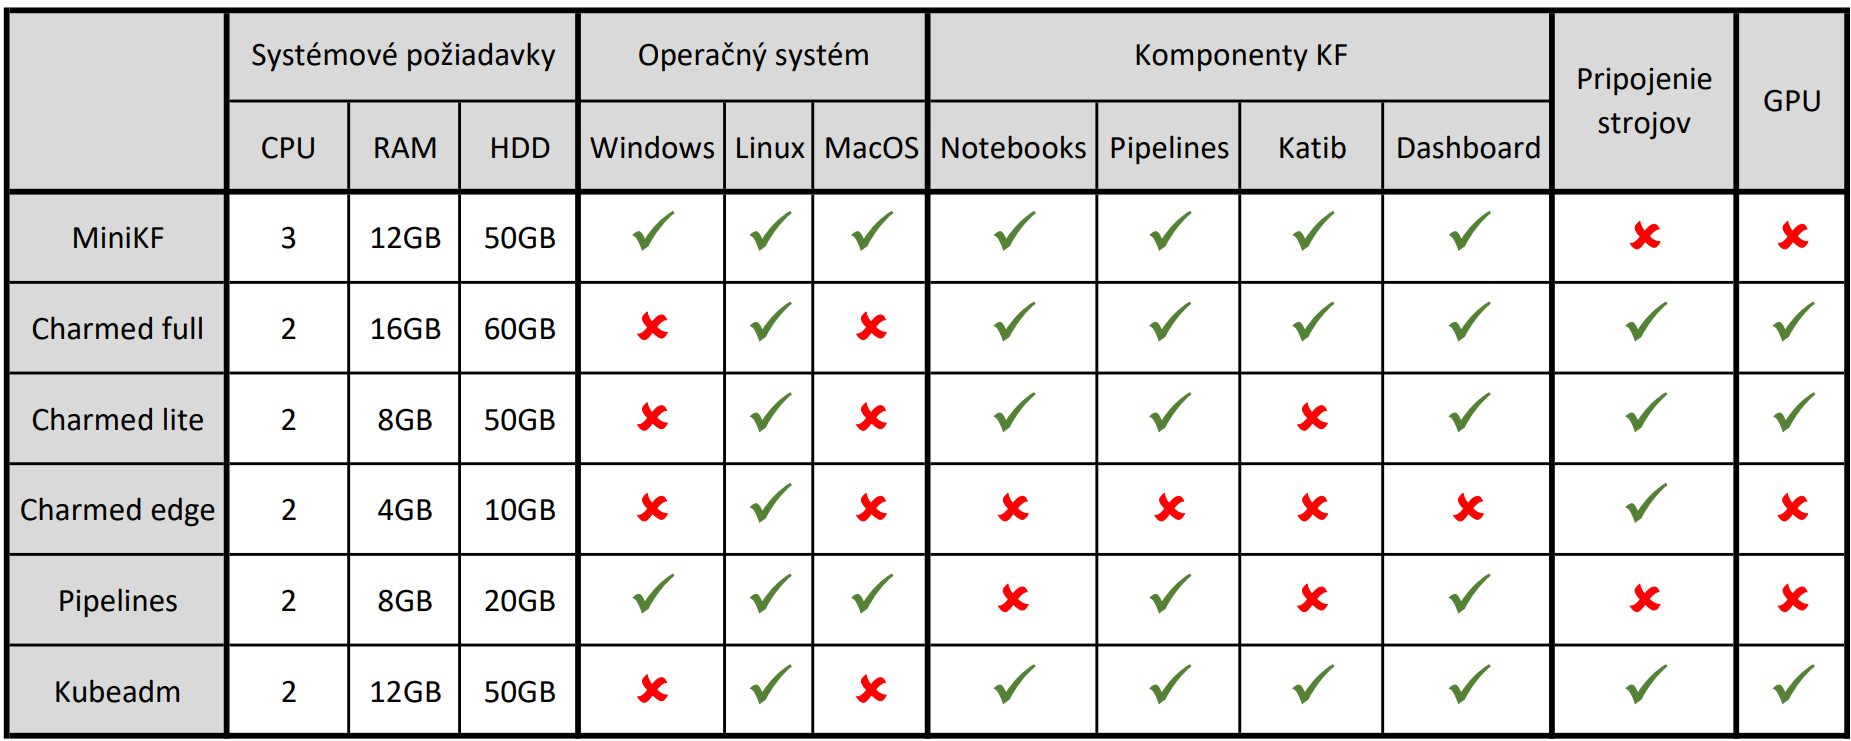
\includegraphics[width=1\linewidth]{figures/table}
    \caption{Požiadavky a funkcie implementácií.}
\end{table}
% !TEX root = ../thesis.tex

\chapter{Záver}
\label{summary}

V tejto bakalárskej práci, bolo prvým krokom analyzovanie a stručný opis platformy Kubernetes, ktorá sa vzhľadom na problematiku tejto práce využíva na riešenie úloh strojového učenia. Čitateľ je oboznámený s výhodami tejto platformy, ktoré ponúka. Za dôležité sa považoval opis a rozdelenie architektúry jednotlivých komponentov, z ktorých je platforma zložená. Sú často spomínane v ďalších kapitolách, preto je vhodné sa s nimi zoznámiť. Porovnané sú niektoré známe nástroje, ktoré sú dostupné na internete na vytvorenie klastra Kubernetes. Kontajnerizácia je neodmysliteľnou súčasťou správnej funkčnosti tejto platformy. Poukazuje na to, aké má výhody oproti virtualizačným systémom a preto je adekvátna na riešenie daného problému.

Na riešenie problémov strojového učenia je najlepším a zároveň najznámejším systémom Kubeflow, slúžiaci na nasadenie pre platformu Kubernetes, ktorý obsahuje všetko pre obľúbencov a inžinierov strojového učenia. Súčasťou je charakteristika dôležitých časti a pracovných postupov pre predstavu o chode tohto systému. Opísane sú postupy na vytvorenie testovacieho prostredia využívajúce tento systém, pre spúšťanie úloh naprogramovaných v jazyku Python. Používateľ je bližšie informovaný o krokoch a postupoch, ktoré sú žiadané a aké požiadavky tento scenár nasadenia vyžaduje od hardvérových až systémových nárokov. V prípade, že scenár podporuje GPU a viacuzlový klaster pri danom scenári je pripojenie strojov alebo podpora grafickej karty.

Na záver sú porovnané a zhodnotené tieto nasadenia s odôvodneným výberom najlepšieho scenára pre splnenie požiadaviek tejto práce. Výsledkom je vytvorený Kubernetes klaster s pripojenými strojmi umožňujúci nasadenie úloh strojového učenia, ktorý sa bude využívať v laboratóriu inteligentných informačných systémov. Obsahuje aj manuál na vytvorenie a pripojenie viacerých počítačov do platformy Kubernetes, a tiež manuál na implementáciu a nasadenie Python zdrojových kódov spustiteľných na platforme Kubernetes.

% good linebraking of bibtex url
\setcounter{biburllcpenalty}{7000}
\setcounter{biburlucpenalty}{8000}

%% The bibliography
\printbibliography[heading=bibintoc]

\label{theend} % the last page of the thesis

% List of acronyms
\printglossary[type=\acronymtype,title={\acrlistname}]

% Glossaries
\printglossary

%% Appendix
% !TEX root = ../thesis.tex

\chapter*{\appendixlistname}
\addcontentsline{toc}{chapter}{\appendixlistname}

\begin{description}
	\item[\appendixname{} A] Systémová príručka
    \item[\appendixname{} A] Používateľská príručka
\end{description}

\appendix
\renewcommand\chaptername{\appendixname}
% !TEX root = ../thesis.tex

\chapter{Karel Language Reference}

\section{Karel's Primitives}

\begin{itemize}
    \item \verb|void movek()| - Moves \textit{Karel} one intersection forward.
    \item \verb|void turn_left()| - Pivots \textit{Karel} $90$ degrees left.
    \item \verb|void pick_beeper()| - Takes a beeper from the current intersection and puts it in the beeper bag.
    \item \verb|void put_beeper()| - Takes a beeper from the beeper bag and puts it at the current intersection.
    \item \verb|void turn_on(char* path)| - Turns \textit{Karel} on.
    \item \verb|void turn_off()| - Turns \textit{Karel} off.
\end{itemize}


\section*{Karel's Sensors}

\begin{itemize}
    \item \verb|int front_is_clear()| - Returns \texttt{1} if there is no wall directly in front of \textit{Karel}. \texttt{0} if there is.
    \item \verb|int right_is_clear()| - Returns \texttt{1} if there is no wall immediately to \textit{Karel}'s right. \texttt{0} if there is.
    \item \verb|int beepers_present()| - Returns \texttt{1} if \textit{Karel} is standing at an intersection that has a beeper. \texttt{0} otherwise.
    \item \verb|int facing_north()| - Returns \texttt{1} if \textit{Karel} is facing north. \texttt{0} otherwise.
    \item \verb|int beepers_in_bag()| - Returns \texttt{1} if there is at least one beeper in \textit{Karel}'s beeper bag. \texttt{0} if the beeper bag is empty.
\end{itemize}


\section*{Misc Functions}

\begin{itemize}
    \item \verb|void set_step_delay(int)| - Sets delay of one \textit{Karel}'s step in miliseconds.
    \item \verb|loop(int)| - Repeats \textit{Karel}'s instruction in a loop.
\end{itemize}


% zivotopis autora
%\curriculumvitae\protect
%Táto časť\/ je nepovinná. Autor tu môže uviesť\/ svoje biografické
%údaje, údaje o~záujmoch, účasti na~projektoch, účasti na~súťažiach,
%získané ocenenia, zahraničné pobyty na~praxi, domácu prax, publikácie
%a~pod.

\end{document}
